%instiki:category: FisicaSubatomica
\chapter{Fermiones}
\label{cha:princ-gauge-local} %noinstiki
%instiki:
%instiki:***
%instiki:
%instiki:[[NotasFS|Tabla de Contenidos]]
%instiki:
%instiki:***
%instiki:
%instiki:* [Ecuaci\'on de klein-Gordon](#ecuacion-de-klein)
%instiki:
%instiki:* [Campos escalares complejos](#camp-escal-compl)
%instiki:
%instiki:* [Invarianza gauge local abeliana](#invar-gauge-local)
%instiki:
%instiki:* [Aplicaci\'on a la mec\'anica cu\'antica](#aplic-la-mecan)
%instiki:
%instiki:* [Invarianza gauge local no abeliana](#invar-gauge-local-2)
%instiki:
%instiki:* [Invarianza gauge local para un grupo semisimple](#invar-gauge-local-1)
%instiki:
%instiki:* [$\Phi$ como un triplete de $SU(2)$](#phi-como-un)
%instiki:
%instiki:* [Problemas](#problemas-3)
%instiki:
%instiki:***
%instiki:

\section{Preliminares}

Para detalles adicionales ver por ejemplo \url{https://indico.cern.ch/event/243629}

\subsection{Representaciones de grupos}

\subsubsection{$\operatorname{SO}(2)$ y $\operatorname{U}(1)$}
Considere el grupo de rotaciones de dos ejes reales $SO(2)$. Una representación matricial corresponde al Grupo de matrices $2\times 2$ ortogonales de determinante 1
\begin{align*}
  R(\theta)=
  \begin{pmatrix}
  \cos\theta &\sin\theta\\  
  -\sin\theta&\cos\theta\\  
  \end{pmatrix},
\end{align*}
donde
\begin{align*}
  \det[R(\theta)]=\cos^2\theta+\sin^2\theta=1\,.
\end{align*}

Para generar esta matriz, podemos usar la matriz de traza nula y hermítica ($n$ entrero)
\begin{align*}
  \tau=&
  \begin{pmatrix}
   0 &-i\\ %0 &-i\\
   i &0\\  %i &0\\ 
  \end{pmatrix},&\tau^{2n}=&  \begin{pmatrix}
   1 &0\\
   0 &1\\ 
  \end{pmatrix},&\tau^{2n+1}=&  \begin{pmatrix}
   0 &-i\\
   i &0\\ 
  \end{pmatrix}.
\end{align*}
Entonces
\begin{align}
\label{eq:so2}
  R(\theta)=\exp \left( i \theta\tau \right)=&\sum_{n=0}^{\infty}\frac{\left(i \theta\tau \right)^{n}}{n!}\nonumber\\
=&\sum_{n=0}^{\infty}(i)^{2n}\frac{\left( \theta\tau \right)^{2n}}{2n!}+\sum_{n=0}^{\infty}(i)^{2n+1}\frac{\left( \theta\tau \right)^{2n+1}}{(2n+1)!}\nonumber\\
  =&\sum_{n=0}^{\infty}(-1)^{n}\frac{\theta^{2n}}{2n!}
  \begin{pmatrix}
    1 & 0\\
    0 & 1\\
  \end{pmatrix}
+\sum_{n=0}^{\infty}i(-1)^{n}\frac{ \theta^{2n+1}}{(2n+1)!}
\begin{pmatrix}
  0 & -i \\
  i & 0
\end{pmatrix}
\nonumber\\
    =&
  \begin{pmatrix}
    \cos\theta & 0\\
    0 & \cos\theta \\
  \end{pmatrix}
+
\begin{pmatrix}
  0 & \sin\theta \\
  -\sin\theta & 0
\end{pmatrix}
\nonumber\\
    =&
  \begin{pmatrix}
    \cos\theta & \sin\theta\\
     -\sin\theta& \cos\theta \\
  \end{pmatrix}
\end{align}
Este grupo es Abeliano, ya que
\begin{align}
  R(\theta_1)R(\theta_2)=R(\theta_2)R(\theta_1)
\end{align}
De otro lado el Grupo $U(1)$ corresponde a las rotaciones de un eje complejo y tiene elementos
\begin{align}
  U(\theta)=e^{i \theta Y}\,,
\end{align}
donde $Y$ es el generador de los elementos del Grupo y su representación es un número real. 

Estos dos grupos son isomorfos: para un elemento complejo $U(\theta)$ el correspondiente elemento en $SO(2)$ es la rotación por el ángulo el cual es el argumento de $U(\theta)$
\subsubsection{$\operatorname{S0}(3)$}
\begin{english}
First, let us consider a simpler group, corresponding to the rotation group in tree dimensions. The generators are the angular momentum operators $J^i$, which satisfy the commutation relations
\end{english}
\begin{spanish}
Consideremos primero un grupo más simple, el correspondiente a las rotaciones en tres dimensiones. 
\end{spanish}
Para conocer las relaciones de conmutación de los generadores del grupo de rotaciones, podemos escribir los generadores como operadores diferenciales; de la expresión 
\begin{align}
  \mathbf{J}=&\mathbf{r}\times \mathbf{p}=\mathbf{r}\times (-i\boldsymbol{\nabla})
\end{align}
o en componentes
\begin{align}
\label{eq:rxpi}
  J^k=\left[\mathbf{x}\times (-i\boldsymbol{\nabla})\right]^k=&
-i\sum_j\epsilon_{ijk}x^i\partial_j=i\epsilon_{ijk}x^i\partial^j\,.
\end{align}

Las relaciones de conmutación del momento angular \eqref{eq:rotgr} se obtienen de forma directa
\begin{align*}
  \left[ J^i,J^j \right]\psi=&-\left[ \epsilon_{ilm}x^{l}\partial_m ,\epsilon_{jpq}x^{p}\partial_q \right]\psi \nonumber\\
=&-\epsilon_{ilm}\epsilon_{jpq}\left[ x^{l}\partial_m ,x^{p}\partial_q \right]\psi \nonumber\\
=&-\epsilon_{ilm}\epsilon_{jpq}\left[ x^{l}\partial_m \left(x^{p}\partial_q\psi  \right)-x^{p}\partial_q \left( x^{l}\partial_m\psi \right) \right] \nonumber\\
   =&-\epsilon_{ilm}\epsilon_{jpq}\left( x^{l}\delta_{mp}\partial_q\psi +x^{l}x^{p}\partial_m \partial_q\psi  -x^{p}\delta_{ql}\partial_m\psi-x^{p}  x^{l}\partial_q\partial_m\psi \right)\,,
\end{align*}
cancelando las derivadas cruzadas
\begin{align*}
\phantom{\left[ J^i,J^j \right]\psi}   =&-\epsilon_{ilm}\epsilon_{jpq}\left( x^{l}\delta_{mp}\partial_q\psi   -x^{p}\delta_{ql}\partial_m\psi \right) \nonumber\\
   =&-\epsilon_{ilm}\epsilon_{jpq} x^{l}\delta_{mp}\partial_q\psi +i\epsilon_{ilm}\epsilon_{jpq}x^{p}\delta_{ql}\partial_m\psi \nonumber\\
   =&-\epsilon_{ilm}\epsilon_{jmq} x^{l}\partial_q\psi +i\epsilon_{ilm}\epsilon_{jpl}x^{p}\partial_m\psi \nonumber\\
   =&-\epsilon_{ilm}\epsilon_{jmq} x^{l}\partial_q\psi +i\epsilon_{iml}\epsilon_{jqm}x^{q}\partial_l\psi \qquad (l\leftrightarrow m)\ \text{in 2nd term}\nonumber\\
   =&-\epsilon_{ilm}\epsilon_{jmq} x^{l}\partial_q\psi +i\epsilon_{imq}\epsilon_{jlm}x^{l}\partial_q\psi  \qquad (l\leftrightarrow q)\ \text{in 2nd term}\,,
\end{align*}
y finalmente
\begin{align*}
  \left[ J^i,J^j \right]\psi  =& \left(-\epsilon_{ilm}\epsilon_{jmq}+\epsilon_{imq}\epsilon_{jlm}  \right) x^{l}\partial_q\psi \nonumber\\
   =& \left(\epsilon_{ilm}\epsilon_{jqm}-\epsilon_{iqm}\epsilon_{jlm}  \right) x^{l}\partial_q\psi \nonumber\\
   =& \left(\cancel{\delta_{ij}\delta_{lq}}-\delta_{iq}\delta_{lj}-\cancel{\delta_{ij}\delta_{ql}}+\delta_{il}\delta_{qj}  \right) x^{l}\partial_q\psi \nonumber\\
  =& \left(\delta_{il}\delta_{qj}-\delta_{iq}\delta_{lj}  \right) x^{l}\partial_q\psi \nonumber\\
  =& \epsilon_{kij}\epsilon_{klq} x^{l}\partial_q\psi \nonumber\\
  =&i \epsilon_{kij}\left(-i\epsilon_{klq} x^{l}\partial_q  \right)\psi \nonumber\\
  =&i \epsilon_{kij}J^{k}\psi \,.
\end{align*}

Por consiguiente, Los generadores son los operadores de momento angular $ J^i$, que satisfacen las relaciones de conmutación
\begin{align}
\label{eq:rotgr}
  \left[J^i,J^j\right]=i\epsilon_{ijk}J^k\,.
\end{align}
donde $\epsilon_{ijk}$ son las constantes de estructura del Grupo $SU(2)$

Una representación matricial de esta álgebra se puede obtener con la llamada representación adjunta del Grupo de rotaciones en 3 dimensiones, $SO(3)$, definida a partir de las constantes de estructura \cite{Veltman}
\begin{align}
  (L^i)_{jk}=-i\epsilon_{ijk}\,.
\end{align}
Explícitamente
\begin{align*}
  L^1=&
  \begin{pmatrix}
   0 & 0 & 0\\
   0 & 0 & -i\\
   0 & i & 0 \\
  \end{pmatrix}&
 L^2=&
 \begin{pmatrix}
  0 & 0  & i \\ 
  0 & 0  & 0 \\
 -i & 0  & 0 \\
 \end{pmatrix}&
 L^3=&
 \begin{pmatrix}
   0 & -i & 0\\
   i & 0  & 0\\
   0 & 0 & 0\\
 \end{pmatrix}
\end{align*}

Estos generan los elementos de $SO(3)$
\begin{align}
  R(\boldsymbol{\theta})=&\exp(i \theta_j L^{j}),\qquad\text{sum in $j$}\nonumber\\
                 =&\exp(i\theta_1 L_1+i\theta_2 L_2+i\theta_3 L_3)\,.
\end{align}

Para aislar los subgrupos de un parámetro definimos:
\begin{align}
  R_i\equiv R(\theta_i)
\end{align}
donde, haciendo los mismos pasos que para $SO(2)$ en \eqref{eq:so2},
\begin{align}
  R(\theta_1)=&
  \begin{pmatrix}
   1 &   0        &0\\
   0 &\cos\theta_1  & \sin\theta_1\\
   0 & -\sin\theta_1& \cos\theta_1\\
  \end{pmatrix},\quad R(\theta_2)=
  \begin{pmatrix}
     \cos\theta_2 &0& -\sin\theta_2\\
     0          &1& 0          \\
    \sin\theta_2  &0&  \cos\theta_2\\
  \end{pmatrix}\quad R(\theta_3)=
  \begin{pmatrix}
     \cos\theta_3 & \sin\theta_3&0\\
     -\sin\theta_3& \cos\theta_3&0\\
      0         &     0     &1\\
  \end{pmatrix}\,,
\end{align}
que corresponden respectivamente a rotaciones sobre el eje $x$ por un ángulo $\theta_1$, sobre el eje $y$ por un ángulo $\theta_2$, sobre el eje $z$ por un ángulo $\theta_3$.

Sin perdida de generalidad, un elemento del grupo $\operatorname{SO}(3)$, es decir, una matriz $3\times3$ ortogonal de determinante 1, $A$, se puede definir como el producto de las anteriores matrices de rotación de un parámetro
\begin{align}
 A =&R(\theta_1)R(\theta_2)R(\theta_3) \nonumber\\
=&
  \begin{pmatrix}
    c_1 c_2-c_3 s_1 s_2    & c_1 c_2 + c_3 c_1 s_2  & s_3 s_2 \\
    -c_1 s_2 - c_3 s_1 s_2 & -s_1 s_2 + c_3 c_1 c_2 & s_3 c_2 \\
    s_3 s_1               & -s_3 c_1               & c_3\\
  \end{pmatrix},
\end{align}
donde $c_i=\cos \theta_i$,  $s_i=\sin \theta_i$.

Claramente, el Grupo $SO(3)$ es no Abeliano, es decir
\begin{align*}
  R(\boldsymbol{\theta}_1)R(\boldsymbol{\theta}_2)\ne R(\boldsymbol{\theta}_2)R(\boldsymbol{\theta}_1)
\end{align*}

Note que la combinación lineal se puede expresar como
\begin{align}
  i\boldsymbol{\theta}\cdot\boldsymbol{L}=& i\theta_1 L_1+i\theta_2 L_2+i\theta_3 L_3 \nonumber\\
=&   \begin{pmatrix}
  0           & \theta_3 & -\theta_2 \\
  -\theta_3   &  0       & \theta_1 \\
  \theta_2    & -\theta_1 & 0
   \end{pmatrix}.
\end{align}

Un ejemplo de vector es el vector de velocidad, $\boldsymbol{v}$. Sea $\boldsymbol{k}$ un vector unitario describiendo un eje de rotación sobre el cual $\boldsymbol{v}$ rota por un ángulo $\theta$ de acuerdo a la regla de la mano derecha como se ilustra en la figura~\ref{fig:rf}.
\begin{figure}
  \centering
  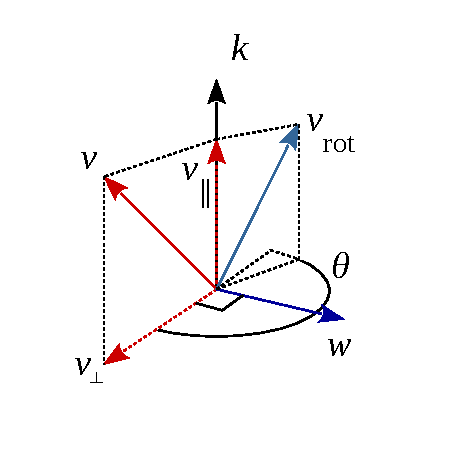
\includegraphics[scale=0.8]{Rodrigues-formula}
  \caption{Rotación vector velocidad. Tomado de \cite{rodriguez}}
  \label{fig:rf}
\end{figure}

Representado el resultado del producto vectorial $\boldsymbol{k}\times\boldsymbol{v}$ como una matrix columna,
\begin{align}
  \begin{pmatrix} (\boldsymbol{k}\times\boldsymbol{v})_x \\ (\boldsymbol{k}\times\boldsymbol{v})_y \\ (\boldsymbol{k}\times\boldsymbol{v})_z \end{pmatrix} = \begin{pmatrix} k_y v_z - k_z v_y \\ k_z v_x - k_x v_z \\ k_x v_y - k_y v_x \end{pmatrix} =& \begin{pmatrix} 0 & -k_z & k_y \\ k_z & 0 & -k_x \\ -k_y & k_x & 0 \end{pmatrix} \begin{pmatrix} v_x \\ v_y \\ v_z \end{pmatrix} \nonumber\\
=& \boldsymbol{K} \boldsymbol{v}\,,
\end{align}
donde
\begin{align}
  \boldsymbol{K}=\begin{pmatrix} 0 & -k_z & k_y \\ k_z & 0 & -k_x \\ -k_y & k_x & 0 \end{pmatrix}
\end{align}
Si definimos la matriz de rotación, $R$ perteneciente a $\operatorname{SO}(3)$, a través de un ángulo $\theta$ sobre el eje $\boldsymbol{k}$
\begin{align}
  R(\theta)=\exp \left( - i \theta i \boldsymbol{K} \right)\,,
\end{align}
entonces
\begin{align}
  R(\theta)=I+ \boldsymbol{K} \sin\theta + (1-\cos\theta)\boldsymbol{K}^2\,.
\end{align}
done $I$ es la matriz identidad. En \cite{rodriguez} se encuentra la demostración.

\subsection{$\operatorname{SU}(2)$} 

La representación matricial isomorfa a $SO(3)$ pero con matrices $2\times2$ corresponde al Grupo $SU(2)$ de rotaciones de dos ejes complejos.
\begin{english}
  The Pauli matrices are set of matrices satisfying this commutation relations:
\end{english}
\begin{spanish}
Las matrices de Pauli son un conjunto de matrices que satisfacen estas mismas condiciones de conmutación: 
\end{spanish}
\begin{equation}
  \label{eq:paulialg}
  \left[\frac{\tau^i}{2},\frac{\tau^j}{2} \right]=i\,\epsilon_{ijk}\frac{\tau^k}{2}
\end{equation}
donde $\tau^i$ 
\begin{equation}
  \label{eq:paulimatr}
  \tau_1=
  \begin{pmatrix}
    0&1\\
    1&0
  \end{pmatrix} \qquad
 \tau_2=
  \begin{pmatrix}
    0&-i\\
    i&0
  \end{pmatrix}\qquad 
 \tau_3=
  \begin{pmatrix}
    1&0\\
    0&-1
  \end{pmatrix}
 \end{equation}
dividas por dos, corresponden a los generadores del Grupo. Las constantes de estructura del Grupo corresponden a $\epsilon_{ijk}$. Como los generadores no conmutan, $SU(2)$ es un Grupo de Lie no Abeliano. Definiendo los generadores de $SU(2)$ como
\begin{equation}
  T^i=\frac{\tau_i}{2},
\end{equation}

Las matrices de Pauli y por consiguiente $T_i$ satisfacen 
\begin{align}
  \tau_i^\dagger&=\tau_i\nonumber\\
  \operatorname{Tr}  \left(
    \tau_i
  \right)&=0
\end{align}
Además
\begin{align}
  \label{eq:64qft}
  \det
  \left(
    \tau_i
  \right)&=-1\nonumber\\
  \left\{ 
    \tau_i,\tau_j
  \right\}&=2\delta_{ij}\cdot I\Rightarrow\tau_i^2=I\nonumber \\
\operatorname{Tr} \left(\tau^i\tau^j\right)&=2\delta^{ij}\nonumber\\
\tau_i\tau_j&=i\epsilon_{ijk}\tau_k+\delta_{ij}\,.
\end{align}

Un elemento del Grupo puede escribirse como
\begin{equation}
  \label{eq:63qft}
  U(\boldsymbol{\theta})=e^{iT^i \theta_i }\approx1+iT^i\theta_i=1+i\frac{\tau^i}{2}\theta_i\,.
\end{equation}
Como antes, $\theta_i$ son los parámetros de la transformación.  Usando las propiedades $T_i$, podemos mostrar que la representación matricial $2\times 2$, $U(\boldsymbol{\theta})$, satisface
\begin{enumerate}
\item Unitariedad: $U^{-1}(\boldsymbol{\theta})=U^{\dagger}(\boldsymbol{\theta})$. En efecto
  \begin{align*}
    U^{\dagger}(\boldsymbol{\theta})U(\boldsymbol{\theta})=&e^{-i{T^i}^{\dagger} \theta_i }e^{iT^i \theta_i }\nonumber\\
=&e^{-i T^i \theta_i }e^{iT^i \theta_i } \nonumber\\
=&e^{\mathbf{0}}\nonumber\\
=&\mathbf{1}\,,
  \end{align*}
la identidad $2\times 2$.
\item Especial (Special): Usando la formula de Jacobi para la exponencial de una matriz, $A$, $e^{A}=e^{\operatorname{Tr}A}$, tenemos que
  \begin{align*}
   \det[U(\boldsymbol{\theta})]=&\det\left\{\exp\left[  i \operatorname{Tr}\left( T^i \right)\theta_i \right]  \right\}\nonumber\\
                           =&e^{0}\nonumber\\
                           =&1\,.
  \end{align*}
\end{enumerate}
De esta manera $T_i$ genera el grupo de matrices $2\times 2$ unitarias y de determinante 1: $SU(2)$. 

El grupo $SU(2)$ de rotaciones de dos ejes complejos, es isomorfo al Grupo $SO(3)$ de rotaciones sobre tres ejes reales.

\subsubsection{$SU(N)$}


En general, si $N^{2}-1$ generadores $\Lambda_i$, satisfacen el álgebra
\begin{align}
  \left[ \Lambda_a,\Lambda_b \right]=f_{abc}\Lambda_{c}\,,
\end{align}
con
\begin{align}
  \Lambda^{\dagger}=&\Lambda\,, & \operatorname{Tr}(\Lambda)=0\,,
\end{align}
entonces las matrices $N\times N$  
\begin{align}
  U(\boldsymbol{\theta})=\exp\left( i \Lambda_{a}\theta_{a} \right)
\end{align}
son unitarias y de determinante 1, y constituyen la representación fundamental de $SU(N)$.

En el caso de $U(1)$, el único generador conmutativo satisface trivialmente el álgebra y da lugar al elemento de grupo
\begin{align}
  U(\theta)=e^{i\Lambda \theta}
\end{align}
que automáticamente tienen norma 1
\begin{align*}
|U(\theta)|^2= U^{*}(\theta)U(\theta)=1\,.
\end{align*}


\section{Grupo de Lorentz }
Para estudiar otros posibles tipos de campos además de los escalares y vectoriales, debemos explorar las representaciones del Grupo de Lorentz en $n$ dimensiones. El grupo de Lorentz es un subgrupo del Grupo de Poincaré que además incluye el subgrupo de las traslaciones en el espacio y el tiempo.

Seguiremos el mismo método de encontrar representaciones matriciales a partir del algebra  de los generadores del Grupo (los cuales deben satisfacer la relaciones de conmutación apropiadas) para luego exponenciar estas representaciones infinitesimales.

\begin{frame}[fragile,allowframebreaks]
Para el presente problema, necesitamos conocer las relaciones de conmutación de los generadores del grupo de transformaciones de Lorentz. Hemos mostrado en la ec.~ \eqref{eq:rotgr}  que, a partir de la relación (haciendo expícito el caracter de operadores)
\begin{align}
\label{eq:rxp}
  \widehat{\mathbf{J}}=&\widehat{\mathbf{r}}\times \widehat{\mathbf{p}}=
\widehat{\mathbf{r}}\times (-i\boldsymbol{\nabla})
\end{align}
la parte correspondiente al grupo de rotaciones es
\begin{align*}
  \left[\widehat{J}^i,\widehat{J}^j\right]=i\epsilon_{ijk}\widehat{J}^k\,.
\end{align*}

La ecuación \eqref{eq:rxp} en términos de componentes esta dada en~\eqref{eq:rxpi} y corresponde a
\begin{align}
  \widehat{J}^k=i\epsilon_{ijk}x^i\partial^j
\end{align}
Definimos una representación matricial de los operadores de momento angular como
\begin{align}
  \widehat{J}^{l m}\equiv\epsilon_{lmk}\widehat{J}^k=&i\epsilon_{lmk}\epsilon_{ijk}x^i\partial^j\nonumber\\
=&i(\delta_{li}\delta_{mj}-\delta_{lj}\delta_{mi})x^i\partial^j\nonumber\\
=&i(x^l\partial^m-x^m\partial^l)\,.
\end{align}
  Que involucran tres generadores. La generalización a cuatro dimensiones da lugar a generadores adicionales $\widehat{J}^{0i}$:
\begin{align}
  \widehat{J}^{\mu\nu}=i(x^\mu\partial^\nu-x^\nu\partial^\mu)\,.
\end{align}
\end{frame}
\begin{frame}[fragile,allowframebreaks]
Los seis generadores satisfacen el álgebra
\begin{align}
\label{eq:lrtalg}
  \left[\widehat{J}^{\mu\nu},\widehat{J}^{\rho\sigma}\right]=&
i(g^{\nu\rho}\widehat{J}^{\mu\sigma}-g^{\mu\rho}\widehat{J}^{\nu\sigma}-g^{\nu\sigma}\widehat{J}^{\mu\rho}+g^{\mu\sigma}\widehat{J}^{\nu\rho})\,.
\end{align}
%From \cite{Peskin}:
Cualquier representación matricial de estos operadores que vaya a representar esta álgebra debe obedecer las mismas reglas de conmutación.


  La exponenciación de los generadores da lugar al grupo de elementos 
\begin{align}
  \widehat{\Lambda}=\exp\left(-i\omega_{\mu\nu}\frac{\widehat{J}^{\mu\nu}}{2}\right)
\end{align}
Para encontrar una representación matricial de los boosts (que son básicamente rotaciones entre el espacio y el tiempo), tenemos
\begin{align}
  \left\{x^\mu\right\}=\begin{pmatrix}
    t\\
    x\\
    y\\
    z
  \end{pmatrix}\to
  \begin{pmatrix}
    t'\\
    x'\\
    y'\\
    z'
  \end{pmatrix}=
  \begin{pmatrix}
    \frac{t+vx}{\sqrt{1-v^2}}\\
    \frac{x+vt}{\sqrt{1-v^2}}\\
    y\\
    z
  \end{pmatrix}=&
  \begin{pmatrix}
    \cosh\xi&\sinh\xi&0&0\\
    \sinh\xi&\cosh\xi&0&0\\
    0     &  0  &1&0\\
    0     &  0  &0&1
  \end{pmatrix}
  \begin{pmatrix}
    t\\
    x\\
    y\\
    z
  \end{pmatrix}\nonumber\\
=&\left\{{\Lambda^\mu}_{\nu}\right\}\left\{x^\nu\right\}\,,
\end{align}
  Ya que
\begin{align}
  \cosh\xi=&\sum_{n=0}^{\infty}\frac{\xi^{2n}}{2n!}\approx 1+\mathcal{O}(\xi^2)\nonumber\\
  \sinh\xi=&\sum_{n=0}^{\infty}\frac{\xi^{2n+1}}{(2n+1)!}\approx \xi+\mathcal{O}(\xi^2)\,,
\end{align}
  Un boost infinitesimal a lo largo de $x$ es
\begin{align}
  \left\{{\Lambda^\mu}_{\nu}\right\}_{x-\text{boost }}\approx
  \begin{pmatrix}
    1&\xi&0&0\\
    \xi&1&0&0\\
    0&0&1&0\\
    0&0&0&1
  \end{pmatrix}=\exp \left( i\xi  K^1 \right),
\end{align}
donde el generador de boost es
\begin{align}
 K^1= \begin{pmatrix}
    0 & -i & 0 & 0\\
   -i & 0  & 0 & 0\\
   0 & 0 &  0 & 0\\
    0 & 0 &  0 & 0\\ 
  \end{pmatrix}.
\end{align}

  Similarmente una rotación por un ángulo infinitesimal $\theta=\theta_3$ alrededor del plano $xy$ (o sobre el eje $z$)
\begin{align}
  \left\{{\Lambda^\mu}_{\nu}\right\}_{xy-\text{rotation }}\approx
  \begin{pmatrix}
    1&0&0&0\\
    0&1&\theta&0\\
    0&-\theta&1&0\\
    0&0&0&1
  \end{pmatrix}.
\end{align}
Que como hemos visto, puede obtenerse a partir de los generadores del Grupo de rotaciones $SO(3)$, generalizados a matrices $4\times4$
\begin{align}
  \{L^{i}\}\equiv
  \begin{pmatrix}
    1 & 0 & 0& 0\\
    0 &   &  &  \\
    0 &   & L^i_{3\times3}  &  \\
    0 &   &  &  \\
  \end{pmatrix}
\end{align}
\begin{align*}
  L^1_{3\times3}=&
  \begin{pmatrix}
   0 & 0 & 0\\
   0 & 0 & -i\\
   0 & i & 0 \\
  \end{pmatrix}&
 L^2_{3\times3}=&
 \begin{pmatrix}
  0 & 0  & i \\ 
  0 & 0  & 0 \\
 -i & 0  & 0 \\
 \end{pmatrix}&
 L^3_{3\times3}=&
 \begin{pmatrix}
   0 & -i & 0\\
   i & 0  & 0\\
   0 & 0 & 0\\
 \end{pmatrix}
\end{align*}.


\end{frame}
En general definimos los seis parámetros independientes del Grupo de Lorentz
\begin{align}
  \omega_{i0}=-\omega_{0i}\equiv&\xi_{i} \nonumber\\
  \omega_{12}=-\omega_{21}\equiv&2\theta^3 &   \omega_{32}=-\omega_{23}\equiv&-2\theta^2 &   \omega_{13}=-\omega_{31}\equiv&2\theta^1\,.
\end{align}
Por lo tanto
\begin{align}
\xi^i=&\omega^{i0}=-\omega^{0i}&\theta^i=&\frac{1}{2}\epsilon^{ijk}\omega_{jk}\,.  
\end{align}

Las  matrices $4\times 4$ 
\begin{align}
   \left(J^{\mu\nu}\right)_{\alpha\beta}=&i\epsilon^{\mu\nu\rho\sigma}\epsilon_{\rho\sigma\alpha\beta}\nonumber\\
   \left(J^{\mu\nu}\right)^{\alpha}_{\beta}=g^{\gamma\alpha}\left(J^{\mu\nu}\right)_{\gamma\beta}= &i\epsilon^{\mu\nu\rho\sigma}\epsilon_{\rho\sigma\gamma\beta}g^{\gamma\alpha}\nonumber\\
\end{align}
\begin{align}
  \left(J^{\mu\nu}\right)_{\alpha\beta}  =&i\left({\delta^\mu}_\alpha{\delta^\nu}_\beta-{\delta^\mu}_\beta{\delta^\nu}_\alpha\right)\nonumber\\
 {\left(J^{\mu\nu}\right)^{\alpha}}_{\beta}=&ig^{\gamma\alpha}\left({\delta^{\mu}}_{\gamma}{\delta^\nu}_\beta-{\delta^\mu}_\beta{\delta^{\nu}}_\gamma\right) \nonumber\\
 =&i\left(g^{\mu\alpha}{\delta^\nu}_\beta-{\delta^\mu}_\beta g^{\nu\alpha}\right)\nonumber\\
{\left(J^{\mu\nu}\right)^{\alpha\beta}}=&i \left( g^{\mu\alpha}g^{\nu\beta}-g^{\mu\beta}g^{\nu\alpha} \right)
\end{align}
where $\mu$ and $\nu$ label which of the six matrices we want, while $\alpha$ and $\beta$ label components of the matrices. These matrices satisfy the commutations relations \eqref{eq:lrtalg}, and generate the three boosts and three rotations of the ordinary Lorentz 4-vectors:
\begin{align}
  {\Lambda^\alpha}_\beta\approx{\delta^\alpha}_\beta-\frac{i}{2}\omega_{\mu\nu}{\left(J^{\mu\nu}\right)^\alpha}_\beta\,.
\end{align}
%ver programa mathematica
En particular
\begin{align*}
  (J^{ij})_{lm}=&i\epsilon^{ij\rho\sigma}\epsilon_{\rho\sigma lm}\\
             =&i\epsilon^{ij\rho 0}\epsilon_{\rho 0 lm}\\
             =&-i\epsilon^{ijk}\epsilon_{klm}\\
             =&\epsilon^{ijk}(L_{k})_{lm}
\end{align*}
o, en términos matriciales
\begin{align}
  L^{i}=\tfrac{1}{2}\epsilon^{ijk}J_{jk}
\end{align}
De modo que
\begin{align}
\label{eq:klkl}
  i\sum_i \theta^{i}L^{i}=-&i\theta^iL_i\nonumber\\
=&- \frac{i}{2}\epsilon^{ikl}\omega_{kl}\frac{1}{2}\epsilon_{imn}J^{mn}\nonumber\\
=&- \frac{i}{4}(\delta^k_m\delta^l_n-\delta^k_n\delta^l_m)\omega_{kl}J^{mn}\nonumber\\
=&- \frac{i}{4}(\omega_{kl}J^{kl}-\omega_{kl}J^{lk})\nonumber\\
=&- \frac{i}{4}(\omega_{kl}J^{kl}+\omega_{kl}J^{kl})\nonumber\\
=&- \frac{i}{2}\omega_{kl}J^{kl}\,.
\end{align}

usando la notación de \cite{0812.1594}, definimos también
\begin{align}
  K^i\equiv J^{0i}=-J^{i0}\,,
\end{align}
Entonces
\begin{align}
-i\omega_{\mu\nu}\frac{\widehat{J}^{\mu\nu}}{2} =&-i\omega_{0\nu}\frac{\widehat{J}^{0\nu}}{2}
-i\omega_{i\nu}\frac{\widehat{J}^{i\nu}}{2}\nonumber\\
=&-i\omega_{0i}\frac{\widehat{J}^{0i}}{2}
-i\omega_{i0}\frac{\widehat{J}^{i0}}{2}
-i\omega_{ij}\frac{\widehat{J}^{ij}}{2}\nonumber\\
=&  -i\omega_{i0}\widehat{J}^{i0}
-i\omega_{ij}\frac{\widehat{J}^{ij}}{2}\nonumber\\
=&  i\omega_{i0}\widehat{J}^{0i}
-i\omega_{ij}\frac{\widehat{J}^{ij}}{2}\,,
\end{align}
y usando \eqref{eq:klkl}
\begin{align}
=&  -i\xi_{i}K^{i}-i\omega_{ij}\frac{\widehat{J}^{ij}}{2}\nonumber\\
=&\sum_i \left(i\xi^i K^i+i\theta^i L^i  \right)\,.
\end{align}
\begin{frame}
Entonces
\begin{align}
  \{\Lambda\}=\exp\left(-i\omega_{\mu\nu}\frac{\widehat{J}^{\mu\nu}}{2}\right)=
\exp\left( i\boldsymbol{\xi}\cdot\mathbf{K}+i\boldsymbol{\theta}\cdot\mathbf{L} \right)\,.
\end{align}


%ver programa mathematica
\end{frame}

\section{2 representaciones $2\times 2$ del Grupo de Lorentz}
\begin{frame}[fragile,allowframebreaks]
Here we focus on the simplest non-trivial irreducible representations of the Lorentz algebra. These are the two-dimensional (inequivalent) representations: $(\frac{1}{2},0)$ and $(0,\frac{1}{2})$. 

\begin{align}
  S(\Lambda)_{\left( \frac{1}{2},0 \right)}=&\exp\left(-i \omega_{\mu\nu}\frac{\sigma^{\mu\nu}}{2}\right)\nonumber
\end{align}
\begin{align}
  \sigma^{\mu\nu}=\frac{i}{4}\left[\sigma^\mu,\overline{\sigma}^\nu\right]\,.
\end{align}
where
\begin{align}
  \sigma^0=&\mathbf{1}_{2\times2},& \sigma^{i}\to \boldsymbol{\sigma}=&(\sigma^1,\sigma^2,\sigma^3)\nonumber\\
  \overline{\sigma}^0=&\mathbf{1}_{2\times2},& \overline{\sigma}^{i}\to \overline{\boldsymbol{\sigma}}=&(-\sigma^1,-\sigma^2,-\sigma^3)
\end{align}
include the Pauli matrices \eqref{eq:paulimatr}.

\end{frame}
\begin{frame}[fragile,allowframebreaks]
Eq. \eqref{eq:4lt}, which yields
\begin{align}
\label{eq:SLet}
  S(\Lambda)_{\left( \frac{1}{2},0 \right)}\equiv S(\Lambda)=
\exp\left( \boldsymbol{\xi}\cdot \frac{\boldsymbol{\sigma}}{2}+i\boldsymbol{\theta}\cdot \frac{\boldsymbol{\sigma}}{2} \right)\,,
\end{align}

La otra representación independiente es
\begin{align}
\label{eq:SLet}
\left[S(\Lambda)\right]^{*} = S(\Lambda)_{\left(0,\frac{1}{2} \right)}\equiv S^{*}(\Lambda)=&
\exp\left( \boldsymbol{\xi}\cdot \frac{\boldsymbol{\sigma}}{2}+i\boldsymbol{\theta}\cdot \frac{\boldsymbol{\sigma}}{2} \right)^{*}\nonumber\\
=&\exp\left( \boldsymbol{\xi}\cdot \frac{\boldsymbol{\sigma}^{*}}{2}-i\boldsymbol{\theta}\cdot \frac{\boldsymbol{\sigma}^{*}}{2} \right)\,.
\end{align}
 
The components of $S(\Lambda)$ will be denoted as ${\left[ S(\Lambda) \right]_{\alpha}}^{\beta}$. In such a case, $S^{*}$ is another independent $2\times2$ representation of the Lorentz Group. It is denoted by $\left( 0,\frac{1}{2}\right)$, and, in order to emphasize the difference, it is convenient to denote their components with dotted indices $\dot{\alpha},\dot{\beta},\cdots$. We can get $S^{*}$ from $S^{\dagger}$.
\end{frame}




\section{Lorentz transformation of the fields}

Note again, that a term like
\begin{align}
\label{eq:nolor}
  \phi^*(x)a^\mu\partial_\mu\phi(x)\,,
\end{align}
does not left the Action invariant. To have a proper formulation of the quantum mechanics through the general equation
\begin{align}
  i\frac{\partial}{\partial t}\psi=\hat{H} \psi\,,  
\end{align}
with some, to be determined, relativistic Hamiltonian operator $\widehat{H}$, we should be able to build a Lagrangian with temporal derivatives of order one. Therefore, the Lorentz invariant requires all the derivatives of order one.  
\begin{frame}[fragile,allowframebreaks]
Consider spinor fields, which transforms as
\begin{align}
\label{eq:184qft}
  \psi_\alpha(x)\to\psi'_\alpha(x)={\left[ S(\Lambda) \right]_\alpha}^\beta\psi_\beta(\Lambda^{-1}x)\,, 
\end{align}
where $S(\Lambda)$ is some spinorial representation of the Lorentz Group. 
\end{frame}
In matricial form, if $\Psi(x)$ is a two-component column vector, 
\begin{align*}
  \Psi=
  \begin{pmatrix}
   \psi_1\\
   \psi_2\\
  \end{pmatrix}
\end{align*}
then, one representation $2\times2$ of the Lorentz Group, denoted with $(\frac{1}{2},0)$, can be written as
\begin{align}
  \Psi(x)\to \Psi'(x)=S\Psi \left(\Lambda^{-1}x  \right).
\end{align}
In such a case, $S^{*}$ is another independent $2\times2$ representation of the Lorentz Group. It is denoted by $\left( 0,\frac{1}{2}\right)$, and, in order to emphasize the difference, it is convenient to denote their components with dotted indices $\dot{\alpha},\dot{\beta},\cdots$. We can get $S^{*}$ from $S^{\dagger}$. In fact, writing out the fields without arguments to avoid clutter, 
\begin{align}
    \Psi^{\dagger}\to \Psi'^{\dagger}=\Psi^{\dagger}S^{\dagger}.
\end{align}
In components, and anticipating the dotted indices for $S^{*}$, we have
\begin{align}
  \left( \psi'_\alpha \right)^{\dagger}=&\left( \psi_\beta \right)^{\dagger}{\left( S^\dagger\right)^{\dot{\beta}}}_{\dot{\alpha}}\nonumber\\
=&\left( \psi_\beta \right)^{\dagger}{\left( S^*\right)_{\dot{\alpha}}}^{\dot{\beta}}\nonumber\\
=&\left( \psi_\beta \right)^{\dagger}{\left( S^*\right)_{\dot{\alpha}}}^{\dot{\beta}}\,,
\end{align}
\begin{frame}[fragile,allowframebreaks]
If we interpret $\left( \psi_\beta \right)^{\dagger}$ as the components of a new column vector transforming under $S^{*}(\Lambda)$, with dotted components
\begin{align}
 \psi_{\dot{\alpha}}^{\dagger}\equiv \left( \psi_\alpha \right)^{\dagger}
\end{align}
then we have
\begin{align}
  {\psi'}_{\dot{\alpha}}^{\dagger}=&{\left[ S^*(\Lambda)\right]_{\dot{\alpha}}}^{\dot{\beta}} \psi_{\dot{\beta}}^{\dagger}\,,
\end{align}
\end{frame}
or in matricial form
\begin{align}
{{\Psi'}^{\dagger}}^{T}=S^{*}{{\Psi}^{\dagger}}^{T}
\end{align}
\begin{align}
  K=&\begin{pmatrix}
    0 & 1\\
    1 & 0\\
  \end{pmatrix}& K^2=&  K=&\begin{pmatrix}
    1 & 0\\
    0 & 1\\
  \end{pmatrix}
\end{align}

\begin{frame}[fragile,allowframebreaks]
In summary we have the following Lorentz's transformation properties for the fields
\begin{align}
   \phi(x)\to \phi'(x')=&\phi(x) && \text{Scalar field,}\nonumber\\
   A^\mu(x)\to {A'}^\mu=&{\Lambda^\mu}_\nu A^\nu(\Lambda^{-1}x)&&\text{Vector field,}\nonumber\\
  \psi_\alpha(x)\to\psi'_\alpha(x)=&{\left[ S(\Lambda) \right]_\alpha}^\beta\psi_\beta(\Lambda^{-1}x)
&& \text{Left-handed spinor field,}\nonumber\\
 {\psi'}_{\dot{\alpha}}^{\dagger}(x)\to  {\psi'}_{\dot{\alpha}}^{\dagger}(x)=&{\left[ S^*(\Lambda)\right]_{\dot{\alpha}}}^{\dot{\beta}} \psi_{\dot{\beta}}^{\dagger}(\Lambda^{-1}x)&& \text{Rigth-handed anti-spinor field,}\,,
 \end{align}
\end{frame}



In the following we use only the dotted and undotted components for
spinors but not the matricial form. 
\begin{frame}[fragile,allowframebreaks]
There are two additional spin-1/2
irreducible representations of the Lorentz group. $\left( S^{-1}
\right)^T$ and $\left( S^{-1} \right)^{\dagger}$, but these are
equivalent to the $\left( \frac{1}{2},0 \right)$ and the $\left(
  0,\frac{1}{2}\right)$ representations repectively. The spinors that
  transform under these representations have raised spinor indices,
  $\psi^{\alpha}$ and $\psi^{\dagger\dot{\alpha}}$, with
  transformation laws
\begin{align}
  \psi^{\alpha}\to {\psi'}^{\alpha}=&{\left[ \left( S^{-1} \right)^T \right]^{\alpha}}_{\beta}\psi^{\beta}\nonumber\\
  \psi^{\dagger\dot{\alpha}}\to {\psi'}^{\dagger\dot{\alpha}}=&{\left[ \left( S^{-1} \right)^\dagger \right]^{\dot{\alpha}}}_{\dot{\beta}}\psi^{\dagger\dot{\beta}}
\end{align}
where
\begin{align}
  \psi^{\dagger\dot{\alpha}}\equiv \left( \psi^\alpha \right)^{\dagger}
\end{align}
If we interpret $\psi$ and $\psi^{\dagger}$ as two-component vectors in this internal space, we can define the scalar product by using the convention of \emph{descending} contracted indices and \emph{ascending} contracted dotted indices
\begin{align}
\label{eq:conven}
  {{}^{\alpha}}\,{}_{\alpha}\qquad \text{and}\qquad {{}_{\dot{\alpha}}}\,{}^{\dot{\alpha}}\,.
\end{align}
In this way the we can define the scalar product between two spinors as
\begin{align}
\psi\psi\equiv  \psi^{\alpha}\psi_{\alpha}\to {\psi'}^{\alpha}{\psi'}_{\alpha}=& {\left[ \left( S^{-1} \right)^T \right]^{\alpha}}_{\beta}\psi^{\beta} {S_\alpha}^\gamma\psi_\gamma \nonumber\\
 =& {\left( S^{-1} \right)_{\beta}}^{\alpha}{S_\alpha}^\gamma\psi^{\beta}\psi_\gamma \nonumber\\
  =& \delta_{\beta}^{\gamma}\psi^{\beta}\psi_\gamma \nonumber\\
  =& \psi^{\beta}\psi_\beta\,.
\end{align}
and similarly
\begin{align}
  \psi^{\dagger}\psi^{\dagger}\equiv {\psi}^{\dagger}_{\dot{\alpha}}{\psi}^{\dagger\dot{\alpha}}
\to &{\psi'}^{\dagger}_{\dot{\alpha}}{\psi'}^{\dagger\dot{\alpha}}\nonumber\\
=&\psi^{\dagger}\psi^{\dagger}\,.
\end{align}
\end{frame}
To construct Lorentz invariant Lagrangians, one needs to first combine products of spinors to make objects that transforms as Lorentz tensors.
When constructing Lorentz  tensors from fermion fields the lowered indices must only be contracted with raised indices following the same convention established in eq.~(\ref{eq:conven}). A contravariant  Lorentz tensor of rank $(n\times n)$  in this space must have an index structure with $n$ undotted (dotted) indices follow by $n$ dotted (undotted) indices, as for example,   $\alpha_1\alpha_2\ldots\alpha_n\dot{\alpha}_1\dot{\alpha}_2\ldots\dot{\alpha}_n$.

\section{Lagrangian}
\label{sec:dirac-equation}
The Scrodinger equation can be written as
\begin{align}
    i\frac{\partial}{\partial t}\psi=\hat{H}_{S} \psi\,,  
\end{align}
where
\begin{align}
  \hat{H}_{S}=\frac{1}{2m}\hat p^2+\widehat V\,.
\end{align}


In order to have a well defined probabilty in relativistic quantum mechanics it is necessary that Lagrangian be linear in the time derivative, in order to obtain the general Sccödinger equation:
\begin{align}
  i\frac{\partial}{\partial t}\psi=\hat{H} \psi\,,  
\end{align}
like the Scrödinger Lagrangian. However, this automatically imply that the Lagrangian will be also linear in the spacial derivatives. A pure scalar field cannot involve a Lorentz invariant term of only first derivatives (see eq.~\eqref{eq:nolor}). Therefore the proposed field must have some internal structure associated with some representation of the Lorentz Group. Therefore we build the Lagrangian for a field of several components
\begin{align}
  \psi=  \begin{pmatrix}
\psi_1\\
\psi_2\\
\vdots\\
\psi_n    
  \end{pmatrix}
\end{align}

\subsection{Lorentz transformation}

If the field is to describe the electron. it must have spin and in this way it must transform under some spin representation of the Lorentz Group
\begin{align}
  \psi(x)\to \psi'(x)=S(\Lambda)\psi\left(\Lambda^{-1}x\right)\,.
\end{align}
We work in the simpler case of $2\times2$ representation of the
Lorentz Group. As the electron has both spin and electric charge, we
need at least 4 degrees of freedom to describe it, or equivalently two
complex numbers: We assume for the following discussion that $\psi$ is
one of this complex numbers.
 
Returning back to the space-time Lorentz transformation 
\begin{align}
\label{eq:4lt}
  \{\Lambda\}=\exp\left(-i\omega_{\mu\nu}\frac{\widehat{J}^{\mu\nu}}{2}\right)=
\exp\left( i\boldsymbol{\xi}\cdot\mathbf{K}+i\boldsymbol{\theta}\cdot\mathbf{L} \right)\,,
\end{align}
Here we focus on the simplest non-trivial irreducible representations of the Lorentz algebra. These are the two-dimensional (inequivalent) representations: $(\frac{1}{2},0)$ and $(0,\frac{1}{2})$. In the $(\frac{1}{2},0)$ representation, $\mathbf{L}=\boldsymbol{\sigma}/2$ and $\mathbf{K}=-i\boldsymbol{\sigma}/2$ in
Eq. \eqref{eq:4lt}, which yields
\begin{align}
\label{eq:SLet}
  S(\Lambda)_{\left( \frac{1}{2},0 \right)}\equiv S(\Lambda)=
\exp\left( \boldsymbol{\xi}\cdot \frac{\boldsymbol{\sigma}}{2}+i\boldsymbol{\theta}\cdot \frac{\boldsymbol{\sigma}}{2} \right)\,,
\end{align}
where $\boldsymbol{\sigma}=(\sigma_1,\sigma_2,\sigma_3)$ are the Pauli matrices \eqref{eq:paulimatr}.

\begin{frame}[fragile,allowframebreaks]
We could need a new representation acting in and internal space upon a
two-component field $\psi_a$ ($a=1,2$). An Action with a Lagrangian term linear in the derivatives, could be Lorentz invariant if, taking into account the convention in eq.~(\ref{eq:conven}) and the dotted-undotted structure of the tensor in this internal space, we have that if $a^{\mu}$ is to be a 2th rank tensor of the internal space, it must have components, e.g, $\left( a^{\mu} \right)^{\dot{\alpha}\beta}$. Therefore, a posible Lorentz invariant with a single derivative could be 
 \begin{align}
   {\psi}^{\dagger}a^\mu\partial_\mu\psi\to  {\psi'}^{\dagger}(x)a^\mu\partial'_\mu\psi'
&={\psi'}^{\dagger}_{\dot{\alpha}}a^{\mu\dot{\alpha}\gamma}{\left(\Lambda^{-1}\right)^\rho}_\mu\partial_\rho \psi'_{\gamma}\,,
\end{align}
with the first letters of the Greek alphabet are used to denote the indices of the internal Lorentz space, and the others the external one. 
\begin{align}
{\psi}^{\dagger}a^\mu\partial_\mu\psi\to  {\psi'}^{\dagger}(x)a^\mu\partial_\mu\psi'
&=
 {S^*_{\dot{\alpha}}}^{\dot{\beta}}{\psi}^{\dagger}_{\dot{\beta}}a^{\mu\dot{\alpha\gamma}}{\left(\Lambda^{-1}\right)^\rho}_\mu\partial_\rho \left( {S_{\gamma}}^{\delta}\psi_\delta \right)\,.
 \end{align} 
As the coordinates $\eta_i$ and $\theta_i$ in eq.~\eqref{eq:SLet} are in the internal Lorentz space, the corresponding Lorentz transformation is constant in the external Lorentz space and
\begin{align}
  {\psi}^{\dagger}a^\mu\partial_\mu\psi\to  {\psi'}^{\dagger}(x)a^\mu\partial_\mu\psi'&=
{\psi}^{\dagger}_{\dot{\beta}}{\left(\Lambda^{-1}\right)^\rho}_\mu {S^{\dagger\dot{\beta}}}_{\dot{\alpha}}a^{\mu\dot{\alpha\gamma}}{S_{\gamma}}^{\delta} \partial_\rho  \psi_\delta \nonumber\\
&=\psi^\dagger {\left(\Lambda^{-1}\right)^\rho}_\mu \left(S^\dagger a^\mu S\right)\partial_\rho\psi\nonumber\\
&=\psi^{\dagger}a^\rho\partial_\rho\psi\,,
\end{align}
if the following condition is satisfied:
\begin{align}
 {\left(\Lambda^{-1}\right)^\rho}_\mu  S^{\dagger}a^\mu S=a^\rho\,,
\end{align}
or
\begin{align}
\label{eq:ltrincond}
{\left(\Lambda\right)^\nu}_\rho{\left(\Lambda^{-1}\right)^\rho}_\mu   S^{\dagger}a^\mu S=&
{\left(\Lambda\right)^\nu}_\rho a^\rho\,,\nonumber\\
\delta^{\nu}_{\mu}   S^{\dagger}a^\mu S=&
{\left(\Lambda\right)^\nu}_\rho a^\rho \nonumber\\
S^{\dagger}a^\nu S=&{\left(\Lambda\right)^\nu}_\rho a^\rho\,,
\end{align}
The only solution is expressed in terms of the $2\times2$ identity and the Pauli matrices
   \begin{align} 
 a^{\mu}=\overline{\sigma}^{\mu}=& \left( \mathbf{1}_{2\times2},\overline{\boldsymbol{\sigma}} \right) \nonumber\\
 =& \left( \sigma^0,\overline{\boldsymbol{\sigma}} \right)\,, 
\end{align}
where
\begin{align}
\sigma^0=& \mathbf{1} & \overline{\boldsymbol{\sigma}}=&-\boldsymbol{\sigma}=\left(-\sigma^1,-\sigma^2,-\sigma^3\right)\,.
\end{align}
\end{frame}
\begin{frame}[fragile,allowframebreaks]
Therefore  the most general Lagrangian for two-component spinors contains at least
\begin{align}
    \mathcal{L}\supset&\frac{i}{2}{\psi}^{\dagger}_{\dot{\alpha}}\left(\overline{\sigma}^{\mu}\right)^{\dot{\alpha}\alpha}\partial_\mu\psi_{\alpha}-m\,\psi^{\alpha}\psi_{\alpha} \nonumber\\
\supset&\frac{i}{2}{\psi}^{\dagger}\overline{\sigma}^\mu\partial_\mu\psi-m\,\psi\psi
\end{align}
To guarantee that $\mathcal{L}^{\dagger}=\mathcal{L}$ so that the Action will be real, the easiest way is to add the hermitian conjugate (h.c) of each of the terms. So that, the most general Lagrangian for one left spinor field is
\begin{align*}
  \mathcal{L}=&\frac{i}{2}{\psi}^{\dagger}\overline{\sigma}^\mu\partial_\mu\psi-m\,\psi\psi+
\text{h.c} \nonumber\\
=&\frac{i}{2}{\psi}^{\dagger}\overline{\sigma}^\mu\partial_\mu\psi-m\,\psi\psi+
\left(\frac{i}{2} {\psi}^{\dagger}\overline{\sigma}^\mu\partial_\mu\psi \right)^{\dagger}-m \left(\psi\psi  \right)^{\dagger}\,,
\end{align*}
and the coefficients have been choosing before hand to give the proper equations of motion. Then,
\begin{align*}
  \mathcal{L}=&\frac{i}{2}{\psi}^{\dagger}\overline{\sigma}^\mu\partial_\mu\psi-\frac{i}{2} \partial_\mu\psi^{\dagger}{\overline{\sigma}^\mu}^{\dagger}\psi-m \left( \psi\psi+\psi^{\dagger}\psi^{\dagger} \right)
\end{align*}
Since
\begin{align}
{\overline{\sigma}^\mu}^{\dagger}=\overline{\sigma}^\mu
\end{align}
as expected to the going to be Pauli matrices, then
\begin{align}
\mathcal{L}=&\frac{i}{2}{\psi}^{\dagger}\overline{\sigma}^\mu\partial_\mu\psi-\frac{i}{2} \partial_\mu \left(  \psi^{\dagger} \overline{\sigma}^\mu\psi\right)
+\frac{i}{2}{\psi}^{\dagger}\overline{\sigma}^\mu\partial_\mu\psi
-m \left( \psi\psi+\psi^{\dagger}\psi^{\dagger} \right)\,,
\end{align}
and dropping out the total derivative, we have finally the most general Action for two-component spinors:
\begin{align}
  \mathcal{L}=&i{\psi}^{\dagger}\overline{\sigma}^\mu\partial_\mu\psi-
m \left( \psi\psi+\psi^{\dagger}\psi^{\dagger} \right)\,.
\end{align}
If $\psi$ have a continuos charge such that
\begin{align}
  \psi\to\psi'=e^{i\alpha}\psi
\end{align}
we can impose that the Lagrangian be invariant under changes of phase of $\psi$. In such a case the mass of the field must be zero and
\begin{align}
   \mathcal{L}=&i{\psi}^{\dagger}\overline{\sigma}^\mu\partial_\mu\psi.
\end{align}

The previous Lagrangian which is invariant under
\begin{align}
  \psi\to \psi'=e^{i\alpha}\psi\,,
\end{align}
is the most general one if $\psi$ have any conserved charge, and will be the one the will use in the subsequent discussions.
\end{frame}


\subsection{Corriente conservada y Lagrangiano de Weyl}
\label{sec:corriente-conservada}
\begin{frame}[fragile,allowframebreaks]
En general
\begin{align}
   J^\mu&\propto\left[\frac{\partial\mathcal{L}}{\partial\left(\partial_\mu\psi\right)}\right]\delta\psi+\delta\psi^\dagger\left[\frac{\partial\mathcal{L}}{\partial\left(\partial_\mu\psi^\dagger\right)}\right]\nonumber\\
   &\propto i\psi^\dagger \overline{\sigma}^\mu(-i\alpha\psi)\nonumber\\
   &\propto i\psi^\dagger \overline{\sigma}^\mu(-i\alpha\psi)\nonumber\\
   &=\psi^\dagger \overline{\sigma}^\mu\psi
\end{align}
y
\begin{equation}
     J^\mu=\psi^\dagger  \overline{\sigma}^\mu\psi\,.
\end{equation}
La  densidad de corriente es
\begin{align}
  J^0&\propto \psi^\dagger \sigma^0\psi=\psi^{\dagger}\psi\,.
\end{align}
Que podemos interpretar como una densidad de probabilidad. Por consiguiente, la ecuación de movimiento se puede interpretar directamente como una ecuación de una función de onda de la mecánica cuántica.
\end{frame}
\subsection{Tensor momento-energía}
\label{sec:tens-momento-energi}
\begin{frame}[fragile,allowframebreaks]
Usando $\sigma^{0}=\mathbf{1}$,
\begin{align}
  T^0_0&=\frac{\partial\mathcal{L}}{\partial\left(\partial_0\psi\right)}\partial_0\psi+\partial_0\psi^\dagger\frac{\partial\mathcal{L}}{\partial\left(\partial_0\psi^\dagger\right)}-\mathcal{L}\nonumber\\
  &=i\psi^\dagger\partial_0\psi-\mathcal{L}\nonumber\\
  &=-i\psi^\dagger \overline{\sigma}^i\partial_i\psi\nonumber\\
  &=-\psi^\dagger \sigma^i \left( -i \partial_i\right)\psi\nonumber\\
  &=-\psi^\dagger(\boldsymbol{\sigma}\cdot\widehat{\mathbf{p}})\psi,\nonumber\\
  \label{eq:118qft}
  &=\psi^\dagger\hat{H}_{W} \psi,
\end{align}
donde hemos definido el Hamiltoniano de Weyl como
\begin{equation}
  \label{eq:denshal}
  \hat{H}_W= -\boldsymbol{\sigma}\cdot\widehat{\mathbf{p}}
\end{equation}
Que corresponde a la proyección del espín en la dirección de movimiento. El signo menos justica la definción de $\psi_{\alpha}$ como un espinor de Weyl izquierdo. Como la ecuación de Scröndinger es de validez general, tenemos entonces que

\begin{equation}
  i\frac{\partial}{\partial t}\psi=\hat{H}_W \psi
\end{equation}
y, como en mecánica clásica usual
\begin{equation}
  \label{eq:99qft}
  \langle\hat{H}_W\rangle=\int \psi^\dagger\hat{H}_W \psi\,d^3x.
\end{equation}
Note que esta relación no es posible para el Hamiltoniado de Weyl con término de masa.

Además
\begin{align}
    T^0_i&=\frac{\partial\mathcal{L}}{\partial\left(\partial_0\psi\right)}\partial_i\psi+\partial_i\psi^\dagger\frac{\partial\mathcal{L}}{\partial\left(\partial_0\psi^\dagger\right)}\nonumber\\
    &=i\psi^\dagger\partial_i\psi\nonumber\\
    &=-\psi^\dagger(-i\partial_i)\psi
\end{align}

de modo que
\begin{align}
\langle\hat{\mathbf{p}}\rangle=\int\psi^\dagger\hat{\mathbf{p}}\psi\,d^3 x
\end{align}
\end{frame}
\subsection{Rigth-handed fermion}

\begin{frame}[fragile,allowframebreaks]
For the right handed two-component field ${\eta^{\dagger}}^{\dot{\alpha}}$ ($\dot{\alpha}=\dot{1},\dot{2}$). a posible Lorentz invariant with a single derivative could be 
 \begin{align}
   {\eta}a^\mu\partial_\mu\eta^{\dagger}\to  {\eta'}\left(a^\mu\right)\partial'_\mu{\eta^{\dagger}}'
&={\eta'}^{\alpha}\left( a^\mu \right)_{\alpha\dot{\alpha}}{\left(\Lambda^{-1}\right)^\nu}_\mu\partial_\nu \,{\eta'}^{\dagger\dot{\alpha}}\nonumber\\
&={\left[ \left( S^{-1} \right)^T \right]^{\alpha}}_{\beta}{\eta}^{\beta}\left( a^\mu \right)_{\alpha\dot{\alpha}}{\left(\Lambda^{-1}\right)^\nu}_\mu {\left[ \left( S^{-1} \right)^\dagger \right]^{\dot{\alpha}}}_{\dot{\beta}}\partial_\nu \,{\eta}^{\dagger\dot{\alpha}}\nonumber\\
&={\left(\Lambda^{-1}\right)^\nu}_\mu{\left[ \left( S^{-1} \right) \right]_{\beta}}^{\alpha}\left( a^\mu \right)_{\alpha\dot{\alpha}}{\left[ \left( S^{-1} \right)^\dagger \right]^{\dot{\alpha}}}_{\dot{\beta}} {\eta}^{\beta}\partial_\nu \,{\eta}^{\dagger\dot{\alpha}}\,.
\end{align}
if the following condition is satisfied:
\begin{align}
\label{eq:ltrincond}
S^{-1}a^\mu \left( S^{-1} \right)^{\dagger}=&{\left(\Lambda\right)^\mu}_\nu a^\nu\,,
\end{align}
The only solution is expressed in terms of the $2\times2$ identity and the Pauli matrices
   \begin{align} 
 a^{\mu}={\sigma}^{\mu} =& \left( \sigma^0,{\boldsymbol{\sigma}} \right)\,, 
\end{align}
and dropping out the total derivative, we have finally the most general Action for two-component spinors:
\begin{align}
  \mathcal{L}=&i{\eta}{\sigma}^\mu\partial_\mu\eta^{\dagger}-
m \left( \eta\eta+\eta^{\dagger}\eta^{\dagger} \right)\,.
\end{align}
con donde hemos definido el Hamiltoniano de Weyl como
\begin{equation}
  \label{eq:denshal}
  \hat{H}_W= \mathbf{\sigma}\cdot\widehat{\mathbf{p}}
\end{equation}
Que corresponde a la proyección del espín en la dirección de movimiento. El signo más justica la definción de $\eta^{\dot{\alpha}}$ como un espinor de Weyl derecho.
\end{frame}

\subsection{Ecuaciones de Euler-Lagrange}
\label{sec:ecuaciones-de-euler}
Queremos que el Lagrangiano de lugar a la ecuación de Scröndinger de validez general
\begin{equation}
  \label{eq:grlsch}
  i\frac{\partial}{\partial t}\psi=\hat{H} \psi
\end{equation}
con el Hamiltoniano dado en la ec.~(\ref{eq:99qft}), que corresponde a un Lagrangiano de sólo derivadas de primer orden y covariante, en lugar del Hamiltoniano para el caso no relativista. 

De hecho, aplicando las ecuaciones de Euler-Lagrange para el campo $\psi^\dagger$ al Lagrangiano en ec.~(\ref{eq:100qft}) ,tenemos
\begin{align}
  \partial_\mu\left[\frac{\partial\mathcal{L}}{\partial\left(\partial_\mu\psi^\dagger\right)}\right]-\frac{\partial\mathcal{L}}{\partial\psi^\dagger}&=0\nonumber\\
  \frac{\partial\mathcal{L}}{\partial\psi^\dagger}&=0\nonumber\\
  \label{eq:114qftm}
  i a^\mu\partial_\mu\psi&=0.
\end{align}
Expandiendo
\begin{align*}
  i \sigma^0\partial_0\psi+i \sigma^i\partial_i\psi&=0\\
  i \sigma^0\partial_0\psi-\boldsymbol\sigma\cdot(-i\boldsymbol{\nabla})\psi&=0,\\
  i \sigma^0\partial_0\psi&=(\boldsymbol\sigma\cdot\hat{\mathbf{p}})\psi,
\end{align*}
Como $\sigma^0=\mathbf{1}$,
\begin{equation}
    i\frac{\partial}{\partial t}\psi=\boldsymbol\sigma\cdot\mathbf{p}\psi.
\end{equation}
De la ec.~(\ref{eq:denshal})
\begin{equation}
  \label{eq:186qft}
  \hat{H}= \boldsymbol\sigma\cdot\mathbf{p},
\end{equation}
A este punto, sólo nos queda por determinar los parámetros $a^\mu$. 

La ec.~(\ref{eq:grlsch}) puede escribirse como
\begin{equation}
  \left(i\frac{\partial}{\partial t}-\hat{H}\right)\psi=0.
\end{equation}
El campo $\psi$ también debe satisfacer la ecuación de Klein-Gordon. Podemos derivar dicha ecuación aplicando el operador
\begin{equation*}
  \left(-i\frac{\partial}{\partial t}-\hat{H}\right)
\end{equation*}
De modo que, teniendo en cuenta que $\partial\hat H/\partial t=0$,
\begin{align}
  \label{eq:105qft}
 \left(-i\frac{\partial}{\partial t}-\hat{H}\right)\left(i\frac{\partial}{\partial t}-\hat{H}\right)\psi&=0\nonumber\\
 \left(-i\frac{\partial}{\partial t}-\hat{H}\right)\left(i\frac{\partial\psi}{\partial t}-\hat{H}\psi\right)&=0\nonumber\\
 \frac{\partial^2\psi}{\partial t^2}+i\left(\frac{\partial\hat{H}}{\partial t}\right)\psi
 +i\hat{H}\frac{\partial\psi}{\partial t}-i\hat{H}\frac{\partial\psi}{\partial t}+\hat{H}^2\psi&=0\nonumber\\
 \left(\frac{\partial^2}{\partial t^2}+\hat{H}^2\right)\psi&=0.
\end{align}
% 
De la ec.~(\ref{eq:186qft}), y usando la condición en ec.~(\ref{eq:gamma02}), tenemos
\begin{align}
\label{eq:106qft}
\hat{H}^2&=(\boldsymbol\sigma\cdot\mathbf{p})(\boldsymbol\sigma\cdot\mathbf{p})\,.
\end{align}

Sea $A$ una matriz y $\theta$ en un escalar. Entonces tenemos la identidad
\begin{align}
  \label{eq:206qft}
  (\mathbf{A}\cdot\boldsymbol{\theta})^2=\sum_i {A^i}^2 {\theta^i}^2+\sum_{i\lt j}\left\{A^i,A^j  \right\}\theta^i \theta^j 
\end{align}
\begin{itemize}
\item \textbf{Demostración}
  \begin{align}
    \left[\left(\mathbf{A}\cdot\boldsymbol{\theta}\right)\right]_{\alpha\beta}
    =&\sum_{i j}\sum_\gamma A^i_{\alpha\gamma}\theta^iA^j_{\gamma\beta}\theta^j\nonumber\\    
    =&\sum_{i j}\theta^i\theta^j\sum_\gamma A^i_{\alpha\gamma}A^j_{\gamma\beta}\nonumber\\    
    =&\sum_\gamma \sum_{i j}\theta^i\theta^jA^i_{\alpha\gamma}A^j_{\gamma\beta}\nonumber\\    
    =&\sum_\gamma \left(\sum_{i}{\theta^i}^2A^i_{\alpha\gamma}A^i_{\gamma\beta}+\sum_{i<j}\theta^i\theta^jA^i_{\alpha\gamma}A^j_{\gamma\beta}+\sum_{i>j}\theta^i\theta^jA^i_{\alpha\gamma}A^j_{\gamma\beta}\right)\nonumber\\    
    =&\sum_\gamma \left(\sum_{i}{\theta^i}^2A^i_{\alpha\gamma}A^i_{\gamma\beta}+\sum_{i<j}\theta^i\theta^jA^i_{\alpha\gamma}A^j_{\gamma\beta}+\sum_{j>i}\theta^j\theta^iA^j_{\alpha\gamma}A^i_{\gamma\beta}\right)\nonumber\\    
    =&\sum_\gamma \left[\sum_{i}{\theta^i}^2A^i_{\alpha\gamma}A^i_{\gamma\beta}+\sum_{i<j}\theta^i\theta^j\left(A^i_{\alpha\gamma}A^j_{\gamma\beta}+A^j_{\alpha\gamma}A^i_{\gamma\beta}\right)\right]\nonumber\\    
    =&\left[\sum_{i}{\theta^i}^2\left(A^iA^i\right)_{\alpha\beta}+\sum_{i<j}\theta^i\theta^j\left\{ A^i,A^j\right\}_{\alpha\beta}\right]\nonumber\\    
    =&\left[\sum_{i}{\theta^i}^2{A^i}^2+\sum_{i<j}\theta^i\theta^j\left\{ A^i,A^j\right\}\right]_{\alpha\beta}\,.
  \end{align}

\end{itemize}
Entonces
\begin{align}
  \hat{H}^2=& \sigma_i^2p_i^2+\sum_{i\lt j}\left\{ \sigma_i, \sigma_j\right\}p_i p_j
\end{align}
(suma sobre índices repetidos). Si
\begin{align}
  \label{eq:107qft}
   \sigma_i^2&=\mathbf{1}\nonumber\\
  \left\{ \sigma_i, \sigma_j\right\}&=0\qquad i\ne j\,.
\end{align}
que se puede resumir en
\begin{align}
  \left\{ \sigma^i,\sigma^j \right\}=&2\delta_{ij} \mathbf{1}\,.
\end{align}
todo consistente con las propiedas de las matrices de Pauli en  \eqref{eq:64qft}. 
De modo que
\begin{equation}
  \hat{H}^2=-\boldsymbol{\nabla}^2\,,
\end{equation}
y reemplazando en la ec.~\eqref{eq:105qft} llegamos a la ecuación de Klein-Gordon para $\psi$
\begin{align}
   \left(\frac{\partial^2}{\partial t^2}-\boldsymbol{\nabla}^2\right)\psi&=0\nonumber\\
   \Box\psi&=0
\end{align}
Debido a la ambigüedad  en el signo, podemos construir dos cuadrivectores independientes
   \begin{align}
 \sigma^{\mu}=& \left( \mathbf{1}_{2\times2},\boldsymbol{\sigma} \right)&
 \overline{\sigma}^{\mu}=& \left( \mathbf{1}_{2\times2},\overline{\boldsymbol{\sigma}} \right)
\end{align}
donde
\begin{align}
  \overline{\boldsymbol{\sigma}}=-\boldsymbol{\sigma}=\left(-\sigma^1,-\sigma^2,-\sigma^3\right)\,.
\end{align}
Como hemos visto, las componentes en el espacio interno son
$\sigma^{\mu}_{\alpha\dot{\alpha}}$ y $\overline{\sigma}^{\mu\;\alpha\dot{\alpha}}$, de modo que  las matrices apropiadas son $\overline{\sigma}^\mu$, y el Lagrangiano  y la ecuación de Weyl, son respectivamente de las ecs.~(\ref{eq:100qft}) y (\ref{eq:114qft})
\begin{align}
  \label{eq:115qft}
  \mathcal{L}=&i\psi^\dagger\overline{\sigma}^\mu\partial_\mu\psi \nonumber\\
      =&i\psi^\dagger_{\dot{\alpha}}\overline{\sigma}^{\mu\; \alpha\dot{\alpha}}\partial_\mu\psi_{\alpha}\,,
\end{align}
que da lugar a la ecuación de movimiento
\begin{equation}
  \label{eq:116qft}
  i\overline{\sigma}^\mu\partial_\mu\psi=0,
\end{equation}
Si $\psi$ no tiene ninguna carga continua se puede adicionar un término de masa (con su correspondiente hermítico conjugado)
\begin{align}
  \mathcal{L}=& i\psi^\dagger\overline{\sigma}^\mu\partial_\mu\psi -m \left( \psi\psi+\psi^{\dagger}\psi^{\dagger} \right)\,.
\end{align}

\subsection*{Ejercicio}

Considere un espinor de Weyl que además tiene una carga continua $U(1)$
  \begin{align}
    \psi\to \psi'=e^{i\alpha}\psi\,,
  \end{align}
de modo que su término de masa esta prohíbido.

Escriba el Lagrangiano más general posible para el campo $\psi$ y un campo escalar complejo $\phi$ que transforma como
\begin{align}
  \phi\to \phi'=e^{-2i\alpha}\phi\,.
\end{align}
con un potencial escalar $V(\phi)$ con ruptura espontánea de la simetría continua $U(1)$. Especifique explícitamente las dimensiones y el carácter positivo o negativo de cada uno de los coeficientes. 

Ayuda: sólo hay un término de interacción posible entre los campos fermiónicos y el campo escalar (más el correspondiente hermítico conjugado).

\hrulefill{}$\blacksquare$

\subsection{Ejercicio}

Para el Lagrangiano del punto anterior, encuentre el espectro de partículas cuando la parte real del campo escalar complejo adquiera un valor esperado de vacío, $v$:
  \begin{align*}
    \phi=\frac{H(x)+v+i J(x)}{\sqrt{2}}
  \end{align*}
y especifique cuales son los campos masivos y cuales quedan sin masas. Note entonces que un fermión sin masa también puede adquirir una masa después de la ruptura espontánea de la simetría, como consecuencia de su interacción con un campo escalar.
\label{item:ssb}

\hrulefill{}$\blacksquare$


\subsection{Lorentz invariance of the Weyl Action}
To show that $S(\Lambda)$ is in fact a Lorentz transformation, it is convinient to write this in covariant form. If we define
\begin{align}
  \sigma^{\mu\nu}=\frac{i}{4}\left[\sigma^\mu,\overline{\sigma}^\nu\right]\,.
\end{align}
We can obtain the proper boost and rotations generators:
\begin{align*}
 \mathbf{K}= \sigma^{0i}=&-i\frac{\sigma}{2}\nonumber\\
 L_{i}=\frac{1}{2}\epsilon_{ijk}\sigma^{jk}=&-4\frac{i}{8}\epsilon_{ijk}\left[\frac{\sigma^j}{2},\frac{\sigma^k}{2}  \right]\nonumber\\
=&-\tfrac{i}{2}\epsilon_{ijk}i\epsilon^{jkl}\frac{\sigma_l}{2}\nonumber\\
=&\tfrac{1}{2}\delta_i^l\sigma_l\nonumber\\
=&\tfrac{1}{2}\sigma_i\,.
\end{align*}
% In fact, the six set of non-zero independently generators are
% \begin{align}
%   \mathcal{S}^{0i}=&\frac{i}{4}\left(\gamma^0\gamma^i-\gamma^i\gamma^0\right)=\frac{i}{2}\gamma^0\gamma^i= i B^i\nonumber\\
%   \mathcal{S}^{i j}=&\frac{i}{4}\left(\gamma^i\gamma^j-\gamma^j\gamma^i\right)=\frac{i}{2}\gamma^i\gamma^j= i R^{i j}\,.
% \end{align}
It is worth notices that in fact $\sigma^{\mu\nu}$ satisfy the Lorentz algebra, and therefore are the generators of the Lorentz group elements:
\begin{align}
  S(\Lambda)=&\exp\left(-i \omega_{\mu\nu}\frac{\sigma^{\mu\nu}}{2}\right)\nonumber\\
  \approx&1-\frac{i}{2} \omega_{\mu\nu}{\sigma^{\mu\nu}}\,.
\end{align}


  Necesitamos satisfacer la siguiente condición
\begin{align}
\label{eq:sss}
  S^\dagger\overline{\sigma}^\mu S=&{\Lambda^\mu}_\nu\overline{\sigma}^\nu
\end{align}
Ahora
\begin{align}
\label{eq:SLet}
  S(\Lambda)_{\left( \frac{1}{2},0 \right)}\equiv S(\Lambda)=
\exp\left( \boldsymbol{\xi}\cdot \frac{\boldsymbol{\sigma}}{2}+i\boldsymbol{\theta}\cdot \frac{\boldsymbol{\sigma}}{2} \right)\,,
\end{align}
y expandiendo \eqref{eq:sss}
\begin{align*}
\left(\mathbf{1}+\boldsymbol{\xi}\cdot \frac{\boldsymbol{\sigma}}{2} -i\boldsymbol{\theta}\cdot \frac{\boldsymbol{\sigma}}{2}  \right)
\overline{\sigma}^{\mu}
\left(\mathbf{1}+\boldsymbol{\xi}\cdot \frac{\boldsymbol{\sigma}}{2} +i\boldsymbol{\theta}\cdot \frac{\boldsymbol{\sigma}}{2}  \right)
=&\left[ \mathbf{1}+i\boldsymbol{\xi}\cdot \mathbf{K}+i\boldsymbol{\theta}\cdot \mathbf{L} \right]^{\mu}_{\ \nu}\overline{\sigma}^\nu \nonumber\\
\left(\overline{\sigma}^{\mu}+\boldsymbol{\xi}\cdot \frac{\boldsymbol{\sigma}}{2}\overline{\sigma}^{\mu} -i\boldsymbol{\theta}\cdot \frac{\boldsymbol{\sigma}}{2}\overline{\sigma}^{\mu}  \right)
\left(\mathbf{1}+\boldsymbol{\xi}\cdot \frac{\boldsymbol{\sigma}}{2} +i\boldsymbol{\theta}\cdot \frac{\boldsymbol{\sigma}}{2}  \right)
=&\left[ \mathbf{1}+i\boldsymbol{\xi}\cdot \mathbf{K}+i\boldsymbol{\theta}\cdot \mathbf{L} \right]^{\mu}_{\ \nu}\overline{\sigma}^\nu \,.
\end{align*}
Hasta primer orden en los parametros $\xi^i$ y $\theta^i$,
\begin{align*}
 \overline{\sigma}^{\mu}+\boldsymbol{\xi}\cdot \left(\overline{\sigma}^{\mu} \frac{\boldsymbol{\sigma}}{2} \right)  +i\boldsymbol{\theta}\cdot \left(\overline{\sigma}^{\mu} \frac{\boldsymbol{\sigma}}{2} \right)+\boldsymbol{\xi}\cdot \frac{\boldsymbol{\sigma}}{2}\overline{\sigma}^{\mu} -i\boldsymbol{\theta}\cdot \frac{\boldsymbol{\sigma}}{2}\overline{\sigma}^{\mu}
 =&\delta^{\mu}_{\nu}\overline{\sigma}^\nu+i\boldsymbol{\xi}\cdot {\mathbf{K}^{\mu}}_{\nu}\overline{\sigma}^\nu+i\boldsymbol{\theta}\cdot {\mathbf{L}^{\mu}}_{\nu}\overline{\sigma}^\nu \nonumber\\
   \overline{\sigma}^{\mu}+\boldsymbol{\xi}\cdot \left(\overline{\sigma}^{\mu}\frac{\boldsymbol{\sigma}}{2}+ \frac{\boldsymbol{\sigma}}{2}\overline{\sigma}^{\mu}\right)  +i\boldsymbol{\theta}\cdot \left(\overline{\sigma}^{\mu} \frac{\boldsymbol{\sigma}}{2}-\frac{\boldsymbol{\sigma}}{2}\overline{\sigma}^{\mu} \right)  
 =&\delta^{\mu}_{\nu}\overline{\sigma}^\nu+i\boldsymbol{\xi}\cdot {\mathbf{K}^{\mu}}_{\nu}\overline{\sigma}^\nu+i\boldsymbol{\theta}\cdot {\mathbf{L}^{\mu}}_{\nu}\overline{\sigma}^\nu \nonumber\\
  \boldsymbol{\xi}\cdot \left(\overline{\sigma}^{\mu}\frac{\boldsymbol{\sigma}}{2}+ \frac{\boldsymbol{\sigma}}{2}\overline{\sigma}^{\mu}\right)  +i\boldsymbol{\theta}\cdot \left(\overline{\sigma}^{\mu} \frac{\boldsymbol{\sigma}}{2}-\frac{\boldsymbol{\sigma}}{2}\overline{\sigma}^{\mu} \right)  
 =&i\boldsymbol{\xi}\cdot {\mathbf{K}^{\mu}}_{\nu}\overline{\sigma}^\nu+i\boldsymbol{\theta}\cdot {\mathbf{L}^{\mu}}_{\nu}\overline{\sigma}^\nu\,.
\end{align*}
Igualando coeficientes
\begin{align*}
\overline{\sigma}^{\mu}\frac{\boldsymbol{\sigma}}{2}+ \frac{\boldsymbol{\sigma}}{2}\overline{\sigma}^{\mu}  =&i{\mathbf{K}^{\mu}}_{\nu}\overline{\sigma}^\nu \nonumber\\
\overline{\sigma}^{\mu} \frac{\boldsymbol{\sigma}}{2}-\frac{\boldsymbol{\sigma}}{2}\overline{\sigma}^{\mu}=&
{\mathbf{L}^{\mu}}_{\nu}\overline{\sigma}^\nu
\end{align*}
La primera ecuación es
\begin{align*}
  \overline{\sigma}^{\mu}\frac{\sigma^i}{2} +\frac{\sigma^i}{2}\overline{\sigma}^{\mu}  =&i{\left[ K^i \right]^{\mu}}_{\nu}\overline{\sigma}^\nu \nonumber\\
 =&i{\left[ J^{0i} \right]^{\mu}}_{\nu}\overline{\sigma}^\nu \nonumber\\
  =&i{\left[ J^{0i} \right]^{\mu}}_{\nu}\overline{\sigma}^\nu \nonumber\\
  =&-\left(g^{0\mu}\delta^i_{\nu} -\delta^0_{\nu}g^{i\mu}  \right)\overline{\sigma}^\nu \nonumber\\
  =&-\left(g^{0\mu}\overline{\sigma}^i -g^{i\mu} \overline{\sigma}^0  \right)\,,
\end{align*}
para $\mu=0$
\begin{align*}
  \overline{\sigma}^{0}\frac{\sigma^i}{2} +\frac{\sigma^i}{2}\overline{\sigma}^{0}=&-\overline{\sigma}^i \nonumber\\
  \sigma^i=\sigma^i\,.
\end{align*}
Para $\mu=j$
\begin{align*}
  -\sigma^{j}\frac{\sigma^i}{2} -\frac{\sigma^i}{2}\sigma^j  =& +g^{ij}\sigma^0\nonumber\\
  -\delta^{ij}\mathbf{1}=-\delta^{ij}\mathbf{1}\,.
\end{align*}
La segunda ecuación es
\begin{align*}
\overline{\sigma}^{\mu} \frac{{\sigma^i}}{2}-\frac{{\sigma^i}}{2}\overline{\sigma}^{\mu}=&{\left(L^i  \right)^{\mu}}_{\nu}\overline{\sigma}^\nu \nonumber\\
 =&-{\left(L_i  \right)^{\mu}}_{\nu}\overline{\sigma}^\nu \nonumber\\
=&-\tfrac{1}{2}\epsilon_{ijk}{\left(J^{jk}  \right)^{\mu}}_{\nu}\overline{\sigma}^\nu \nonumber\\
 =&-\tfrac{i}{2}\epsilon_{ijk}\left(g^{j\mu}\delta^{k}_{\nu}-\delta^{j}_{\nu}g^{k\mu}  \right)\overline{\sigma}^\nu \nonumber\\
 =&-\tfrac{i}{2}\epsilon_{ijk}\left(g^{j\mu}\overline{\sigma}^k-g^{k\mu}\overline{\sigma}^j  \right) \nonumber\\
 =&\tfrac{i}{2}\epsilon_{ijk}\left(g^{j\mu}{\sigma}^k-g^{k\mu}{\sigma}^j  \right)\,.
\end{align*}
Para $\mu=0$
\begin{align*}
  \overline{\sigma}^{0} \frac{{\sigma^i}}{2}-\frac{{\sigma^i}}{2}\overline{\sigma}^{0}=& \frac{i}{2}\epsilon_{ijk}\left(g^{j0}{\sigma}^k-g^{k0}{\sigma}^j  \right)\nonumber\\
0=&0 \,.
\end{align*}
Para $\mu=l$
\begin{align*}
  \overline{\sigma}^l \frac{{\sigma^i}}{2}-\frac{{\sigma^i}}{2}\overline{\sigma}^l=&\frac{i}{2}\epsilon_{ijk}\left(g^{jl}{\sigma}^k-g^{kl}{\sigma}^j  \right)\nonumber\\
   \frac{{\sigma^i}}{2}{\sigma}^l -{\sigma}^l \frac{{\sigma^i}}{2}=&\frac{i}{2}\epsilon_{ijk}\left(-\delta^{jl}{\sigma}^k+\delta^{kl}{\sigma}^j  \right)\nonumber\\
  2\frac{\sigma^i}{2}\frac{\sigma^l}{2} -2\frac{\sigma^l}{2}\frac{\sigma^i}{2}=&\frac{i}{2}\left(-\epsilon_{ilk}{\sigma}^k+\epsilon_{ijl}{\sigma}^j  \right)\nonumber\\
 2\left[ \frac{\sigma^i}{2},\frac{\sigma^l}{2} \right]=&\frac{i}{2}\left(\epsilon_{lik}{\sigma}^k+\epsilon_{lik}{\sigma}^k  \right)\nonumber\\
 2i\epsilon_{lik}\frac{\sigma^{k}}{2}=&\frac{i}{2}\left(2\epsilon_{lik}  \sigma^{k}\right)\nonumber\\
 i\epsilon_{lik}{\sigma^{k}}=&i\epsilon_{lik}  \sigma^{k}\,.
\end{align*}


\section{Masas para fermiones de Weyl}
Es interesante notar que el mismo mecanismo que funciona para dar masa a un bosón gauge también puede permitir la aparición de un término de masa para un fermión de Weyl. Considere un fermión de Weyl izquierdo $\psi$ con una cierta carga, que por simplicidad, consideraremos conservada globalmente. Si ademas permitimos la presencia de un escalar complejo, $\phi$, con el doble de dicha carga, tal que
\begin{align}
  \psi\to \psi'=&e^{i\alpha}\psi \nonumber\\
  \phi\to \phi'=&e^{-2i\alpha}\phi\,,
\end{align}
entonce el Lagrangiano más general posible para los dos campos es
\begin{align}
  \mathcal{L}=i\psi^{\dagger}\overline{\sigma}^{\mu}\partial_{\mu}\psi-h \left( \psi\psi\phi+\phi^{*}\psi^{\dagger}\psi^{\dagger} \right)
+\partial^{\mu}\phi\partial_{\mu}\phi-\mu^2 \phi^{*}\phi-\lambda \left( \phi^{*}\phi \right)^{2}\,.
\end{align}
Es importante notar a este punto que el acomplamiento $h$, llamado acoplamiento de Yukawa, es adimensional. Si imponemos además las condiciones $\mu^2<0$ y $\lambda>0$. podemos analizar el espectro de la teoría cerca al mínimo $\left\langle \phi \right\rangle=v$, haciendo el cambio de variables a
\begin{align}
  \phi(x)=\frac{H(x)+v+i J(x)}{\sqrt{2}}\,,
\end{align}
\begin{align*}
   \mathcal{L}=&i\psi^{\dagger}\overline{\sigma}^{\mu}\partial_{\mu}\psi-\frac{h v}{\sqrt{2}} \left( \psi\psi +\psi^{\dagger}\psi^{\dagger} \right)
-\frac{h }{\sqrt{2}} \left( \psi\psi +\psi^{\dagger}\psi^{\dagger} \right)H-i\frac{h }{\sqrt{2}} \left( \psi\psi -\psi^{\dagger}\psi^{\dagger} \right)J \nonumber\\
&+\frac{1}{2}\partial^{\mu} H\partial_{\mu} H+\frac{1}{2}\partial^{\mu} J\partial_{\mu} J-\frac{\mu^2}{2} \left[(H+v)^2+J^2\right]-\frac{\lambda}{4} \left[(H+v)^2+J^2\right]^2 \nonumber\\
               =&i\psi^{\dagger}\overline{\sigma}^{\mu}\partial_{\mu}\psi-m \left( \psi\psi +\psi^{\dagger}\psi^{\dagger} \right)-\frac{m}{v} \left( \psi\psi H  +\psi^{\dagger}\psi^{\dagger}H +i\psi\psi J -i\psi^{\dagger}\psi^{\dagger}J \right) \nonumber\\
&+\tfrac{1}{2}\partial^{\mu} H\partial_{\mu} H-\tfrac{1}{2}\mu^2(H+v)^2-\tfrac{1}{4}\lambda (H+v)^4  \nonumber\\
&+\tfrac{1}{2}\partial^{\mu} J\partial_{\mu} J+\frac{1}{2}\left| \mu^2 \right| J^2-\tfrac{1}{4}\lambda \left[2J^2 \left( H^2+2vH+v^2 \right)+J^4\,\right],
\end{align*}
Usando 
\begin{align*}
  m_H^2=2\left|\mu^2\right|=2\lambda v^2  >0\,,
\end{align*}
tenemos
\begin{align}
   \mathcal{L}=&i\psi^{\dagger}\overline{\sigma}^{\mu}\partial_{\mu}\psi-m \left( \psi\psi +\psi^{\dagger}\psi^{\dagger} \right)-\frac{m}{v} \left( \psi\psi H  +\psi^{\dagger}\psi^{\dagger}H +i\psi\psi J -i\psi^{\dagger}\psi^{\dagger}J \right) \nonumber\\
&+\frac{1}{2}\partial^{\mu} H\partial_{\mu} H-\frac{1}{2}m_H^2H^2-\frac{1}{2}\frac{m_H^2}{v}H^3-\frac{1}{8}\frac{m_H^2}{v^2} H^4 \nonumber\\
&+\frac{1}{2}\partial^{\mu} J\partial_{\mu} J+\cancel{\frac{1}{4} m_H^2 J^2}-\cancel{\frac{1}{4} m_H^2 J^2}- \frac{1}{8}\frac{m_H^2}{v^2} J^4 
-\frac{1}{2}\frac{m_H^2}{v} J^2H -\frac{1}{4}\frac{m_H^2}{v^2} J^2H^2 \nonumber\\
=&i\psi^{\dagger}\overline{\sigma}^{\mu}\partial_{\mu}\psi-m \left( \psi\psi +\psi^{\dagger}\psi^{\dagger} \right)-\frac{m}{v} \left( \psi\psi H  +\psi^{\dagger}\psi^{\dagger}H +i\psi\psi J -i\psi^{\dagger}\psi^{\dagger}J \right) \nonumber\\
&+\frac{1}{2}\partial^{\mu} H\partial_{\mu} H-\frac{1}{2}m_H^2H^2-\frac{1}{2}\frac{m_H^2}{v}H^3-\frac{1}{8}\frac{m_H^2}{v^2} H^4 \nonumber\\
&+\frac{1}{2}\partial^{\mu} J\partial_{\mu} J-\frac{1}{8}\frac{m_H^2}{v^2} J^4 \nonumber\\
&-\frac{1}{2}\frac{m_H^2}{v} J^2H -\frac{1}{4}\frac{m_H^2}{v^2} J^2H^2\,.
\end{align}
El espectro de partículas alrededor del mínimo asociado a la ruptura espontánea de la simetría corresponde a fermión de Weyl con masa (como podría ser por ejemplo un neutrino izquierdo masivo)
\begin{align*}
  m=\frac{hv}{\sqrt{2}}\,,
\end{align*}
un Higgs con masa $m_H^2$ y un bosón de Goldston sin masa $J(x)$. Cuando el bosón de Goldstone no puede ser reabsorvido como la masa de un bosón gauge, corresponde a una partícula física que se suele llamar el Majoron. El término de interacción $\psi \psi J$ implica que un par de fermiones de Weyl se pueden aniquilar en un Majoron (sin masa). Este tipo de procesos están fuertemente suprimidos a partir de observaciones astrofísicas pues podrían implicar por ejemplo un enfriamiento demasiado rápido de una supernova por energía perdida a través de Majorones provenientes de la aniquilación de neutrinos. 


\section{Espinores de Dirac}

Para ir de un cuadrivector de spín barrado al sin barrar
   \begin{align}
 \overline{\sigma}^{\mu}=\left( \mathbf{1}_{2\times2},-{\boldsymbol{\sigma}} \right) \rightarrow
\sigma^{\mu}= \left( \mathbf{1}_{2\times2},\boldsymbol{\sigma} \right)
\end{align}
podemos usar la \emph{métrica de Weyl}
\begin{align}
  \left( \sigma^{\mu} \right)_{\alpha\dot{\alpha}}=&\epsilon_{\alpha\beta}\epsilon_{\dot{\alpha}\dot{\beta}}\overline{\sigma}^{\mu\ \dot{\beta}\beta} \nonumber\\
  \left( \overline{\sigma}^{\mu} \right)^{\mu\;\dot{\alpha}\alpha}=&\epsilon^{\alpha\beta}\epsilon^{\dot{\alpha}\dot{\beta}}{\sigma}^{\mu}_{\beta\dot{\beta}} \,,
\end{align}
Estas expresiones se pueden comprobar explicitamente. Por ejemplo, en el caso de la primera matriz de Pauli
\begin{align*}
  \overline{\sigma}^{1}=
  \begin{pmatrix}
   0 & 1\\
   1 & 0 
  \end{pmatrix}=
  \begin{pmatrix}
   0                                         &\left[\overline{\sigma}^1 \right]^{\dot{1}2}\\
 \left[\overline{\sigma}^1 \right]^{\dot{2}1}&0
  \end{pmatrix}=&
  \begin{pmatrix}
   0                                         &\left[\overline{\sigma}^1 \right]^{\dot{1}2}\\
 \left[\overline{\sigma}^1 \right]^{\dot{2}1}&0
  \end{pmatrix}\nonumber\\
=&\begin{pmatrix}
   0                                         &\epsilon^{2\beta}\epsilon^{\dot{1}\dot{\beta}}\left[\sigma^1 \right]_{\beta\dot{\beta}}\\
\epsilon^{1\beta}\epsilon^{\dot{2}\dot{\beta}} \left[\sigma^1 \right]_{\beta\dot{\beta}}&0
  \end{pmatrix}\nonumber\\
=&\begin{pmatrix}
   0                                         &\epsilon^{21}\epsilon^{\dot{1}\dot{2}}\left[\sigma^1 \right]_{1\dot{2}}\\
\epsilon^{12}\epsilon^{\dot{2}\dot{1}} \left[\sigma^1 \right]_{2\dot{1}}&0
  \end{pmatrix}\nonumber\\
=&\begin{pmatrix}
   0                                         &-\left[\sigma^1 \right]_{1\dot{2}}\\
-\left[\sigma^1 \right]_{2\dot{1}}&0
  \end{pmatrix}\nonumber\\
=&\begin{pmatrix}
   0                                         &-1\\
-1&0
  \end{pmatrix}\nonumber\\
=&-\sigma^1\,.
\end{align*}

Con esto podemos reescribir el siguiente producto de espinores  de Weyl que transforma como un vector en el espacio externo de Lorentz
\begin{align}
\label{eq:exxe}
  \xi^{\dagger}\overline{\sigma}^{\mu}\eta=& \xi^{\dagger}_{\dot{\alpha}}\overline{\sigma}^{\mu\;\dot{\alpha}\alpha}\eta_{\alpha}\nonumber\\
=&\xi^{\dagger}_{\dot{\alpha}}\epsilon^{\alpha\beta}\epsilon^{\dot{\alpha}\dot{\beta}}{\sigma}^{\mu}_{\beta\dot{\beta}} \eta_{\alpha}\nonumber\\
  =&\epsilon^{\dot{\alpha}\dot{\beta}}\xi^{\dagger}_{\dot{\alpha}}{\sigma}^{\mu}_{\beta\dot{\beta}} \epsilon^{\alpha\beta}\eta_{\alpha}\nonumber\\
  =&\xi^{\dagger\;\dot{\beta}}{\sigma}^{\mu}_{\beta\dot{\beta}} \eta^{\beta}\nonumber\\
  =&\pm\eta^{\beta}{\sigma}^{\mu}_{\beta\dot{\beta}}\xi^{\dagger\;\dot{\beta}} \nonumber\\
  =&\pm\eta\,{\sigma}^{\mu}\,\xi^{\dagger} \,,
\end{align}
donde el signo $+$ ($-$) es para campos clásicos (anticonmutantes).
\begin{frame}[fragile,allowframebreaks]
Para describir completamente un electrón, que conserva carga eléctrica bajo $U(1)$, necesitamos todas las componentes detalladas en la Tabla~\ref{tab:electron}
\begin{table}
  \centering
  \begin{tabular}{llll}
    Nombre & Símbolo & Lorentz & $U(1)$\\\hline
    $e_L$: electrón izquierdo & $\xi_{\alpha}$ & ${\left[ S \right]_{\alpha}}^{\beta}$ & $e^{i\theta}$\\
   $\left( e_L \right)^{\dagger}=e^{\dagger}_R$: positrón derecho   & $\left( \xi_{\alpha} \right)^{\dagger}=\xi^{\dagger}_{\dot{\alpha}}$ & ${\left[{S^{*}}\right]_{\dot{\alpha}}}^{\dot{\beta}}$ & $e^{-i\theta}$\\
   $e_R$: electrón derecho   & $\left( \eta^{\alpha} \right)^{\dagger}=\eta^{\dagger\;\dot{\alpha}}$ & ${\left[ \left( S^{-1} \right)^\dagger \right]^{\dot{\alpha}}}_{\dot{\beta}}$& $e^{i\theta}$\\
   $\left( e_R \right)^{\dagger}=e^{\dagger}_L$: positrón izquierdo&$\eta^{\alpha}$& ${\left[ \left( S^{-1} \right)^T \right]^{\alpha}}_{\beta}$ & $e^{-i\theta}$\\\hline
  \end{tabular}
  \caption{Componentes del electrón}
  \label{tab:electron}
\end{table}

\end{frame}
\begin{frame}[fragile,allowframebreaks]
Podemos especificar el Lagrangiano completo para el electrón invariante bajo $U(1)$ sin perdidad de generalidad, usando los dos fermiones izquierdos de cargas opuestas, $\xi_{\alpha}$ y $\eta^{\alpha}$:
\begin{align}
  \xi\to\xi'=&e^{i\theta}\xi &   \eta\to\eta'=&e^{-i\theta}\eta &
\end{align}
como
\begin{align}
\label{eq:dwlag}
  \mathcal{L}=&i\xi^{\dagger}_{\dot{\alpha}}\overline{\sigma}^{\mu\;\dot{\alpha}\alpha}\partial_{\mu}\xi_{\alpha}+i\eta^{\alpha}\sigma^{\mu}_{\alpha\dot{\alpha}}\partial_{\mu}\eta^{\dagger\;\dot{\alpha}}
-m \left(\eta^{\alpha} \xi_{\alpha}+\xi^{\dagger}_{\dot{\alpha}} \eta^{\dagger\;\dot{\alpha}}\right)\nonumber\\
=&i\xi^{\dagger}\overline{\sigma}^{\mu}\partial_{\mu}\xi+i\eta\sigma^{\mu}\partial_{\mu}\eta^{\dagger}
-m \left(\eta\xi+\xi^{\dagger}\eta^{\dagger} \right)\,.
\end{align}
Definiendo el \emph{espinor de Dirac}  y su hermítico conjugado como
\begin{align}
\label{eq:psid}
  \Psi\equiv&  \begin{pmatrix}
   e_L\\
   e_R\\    
  \end{pmatrix}=
  \begin{pmatrix}
   \xi_{\alpha}\\
   \eta^{\dagger\;\dot{\alpha}}    
  \end{pmatrix}&  \Psi^{\dagger}=&
  \begin{pmatrix}
   \left( \xi_{\alpha} \right)^{\dagger} & \left( \eta^{\dagger\;\dot{\alpha}} \right)^{\dagger}    
  \end{pmatrix}=  \begin{pmatrix}
  \xi^{\dagger}_{\dot{\alpha}}& \eta^{\alpha}
  \end{pmatrix}
\end{align}
y usando \eqref{eq:exxe}, tenemos en primer lugar que
\begin{align}
\label{eq:psidm}
  \begin{pmatrix}
  \xi^{\dagger}_{\dot{\alpha}}& \eta^{\alpha}
  \end{pmatrix}
  \begin{pmatrix}
    0           &\mathbf{1}\\
    \mathbf{1} &0\\
  \end{pmatrix} \begin{pmatrix}
   \xi_{\alpha}\\
   \eta^{\dagger\;\dot{\alpha}}    
  \end{pmatrix}
=&
\begin{pmatrix}
  \eta^{\alpha} & \xi^{\dagger}_{\dot{\alpha}}
\end{pmatrix}
\begin{pmatrix}
   \xi_{\alpha}\\
   \eta^{\dagger\;\dot{\alpha}}    
  \end{pmatrix}
\nonumber\\
=&\eta^{\alpha}\xi_{\alpha} +\xi^{\dagger}_{\dot{\alpha}}\eta^{\dagger\;\dot{\alpha}}\nonumber\\
=&\eta\xi+\xi^{\dagger}\eta^{\dagger}\,,
\end{align}
mientras que para los términos cinéticos
\begin{align}
\label{eq:psidd}
  \begin{pmatrix}
  \xi^{\dagger}_{\dot{\alpha}}& \eta^{\alpha}
  \end{pmatrix}
 \begin{pmatrix}
    0           &\mathbf{1}\\
    \mathbf{1} &0\\
  \end{pmatrix}
  \begin{pmatrix}
    0           &\sigma^{\mu}_{\alpha\dot{\alpha}}\\
    \overline{\sigma}^{\mu\;\dot{\alpha}\alpha} &0\\
  \end{pmatrix} \begin{pmatrix}
   \partial_{\mu}\xi_{\alpha}\\
   \partial_{\mu}\eta^{\dagger\;\dot{\alpha}}    
  \end{pmatrix}
=&
 \begin{pmatrix}
  \xi^{\dagger}_{\dot{\alpha}}& \eta^{\alpha}
  \end{pmatrix}
  \begin{pmatrix}
    \overline{\sigma}^{\mu\;\dot{\alpha}\alpha}&0\\
     0                    &\sigma^{\mu}_{\alpha\dot{\alpha}}\\
  \end{pmatrix} \begin{pmatrix}
   \partial_{\mu}\xi_{\alpha}\\
   \partial_{\mu}\eta^{\dagger\;\dot{\alpha}}    
  \end{pmatrix}\nonumber\\
=&\xi^{\dagger}_{\dot{\alpha}}\overline{\sigma}^{\mu\;\dot{\alpha}\alpha}\partial_{\mu}\xi_{\alpha}+\eta^{\alpha}\sigma^{\mu}_{\alpha\dot{\alpha}}\partial_{\mu}\eta^{\dagger\;\dot{\alpha}}\nonumber\\
=&\xi^{\dagger}\overline{\sigma}^{\mu}\partial_{\mu}\xi+\eta\sigma^{\mu}\partial_{\mu}\eta^{\dagger}\,.
\end{align}
Definiendo las matrices de Dirac (en la representación quiral) como
\begin{align}
  \gamma^\mu= \begin{pmatrix}
    0           &\sigma^{\mu}\\
    \overline{\sigma}^{\mu} &0\\
  \end{pmatrix},
\end{align}
las cuales satisfacen el algebra
\begin{align}
  \left\{ \gamma^{\mu},\gamma^{\nu} \right\}=2 g^{\mu\nu}\mathbf{1}\,.
\end{align}

tememos en particular que, 
\begin{align}
  \gamma^0= \begin{pmatrix}
    0           &\mathbf{1}\\
    \mathbf{1} &0\\
  \end{pmatrix}
\end{align}
tal que
\begin{align}
  \left( \gamma^{0} \right)^2=\mathbf{1}_{\text{4$\times 4$}}\,.
\end{align}
Usando (\ref{eq:psid}), (\ref{eq:psidm}) y (\ref{eq:psidd})
\begin{align}
  \mathcal{L}=&i\xi^{\dagger}\overline{\sigma}^{\mu}\partial_{\mu}\xi+i\eta\sigma^{\mu}\partial_{\mu}\eta^{\dagger}
-m \left(\eta\xi+\xi^{\dagger}\eta^{\dagger} \right)\nonumber\\
=&i\Psi^{\dagger}\gamma^{0}\gamma^{\mu}\partial_{\mu}\Psi-m\Psi^{\dagger}\gamma^{0}\Psi\,.
\end{align}
Definiendo finalmente el \emph{espinor de Dirac adjunto}
\begin{align}
  \overline{\Psi}=\Psi^{\dagger}\gamma^{0}\,,
\end{align}
podemos escribir finalmente el Lagrangiano para espinores de Dirac  como
\begin{align}
\label{eq:115qftnew}
  \mathcal{L}=&i\overline{\Psi}\gamma^{\mu}\partial_{\mu}\Psi-m\overline{\Psi}\Psi\,.
\end{align}
\end{frame}
En adelante para simplificar la notación nos referiremos al electrón de Dirac simplemente como $\psi$.

En términos de los campos de Weyl un escalar y un vector de espinores Dirac se escriben como
\begin{align}
\label{eq:mwd}
  \overline{\Psi}\Psi =& \left( e_R \right)^\dagger e_L+\left( e_L \right)^{\dagger}e_R \nonumber\\
  \overline{\Psi}\gamma^{\mu}\Psi=& (e_L)^{\dagger}\overline{\sigma}^{\mu}e_L+(e_R)^{\dagger}\sigma^{\mu}e_{R}\,,
\end{align}


Un tratamiento de la invarianza de Lorentz para la Acción de Dirac esta dado en el Apéndice~\ref{cha:dirac-action}. 

\begin{frame}[fragile,allowframebreaks]
La ecuación de Dirac se obtiene facilmente de la ecuación de Euler Lagrange para el espinor adjunto $\overline{\Psi}$
\begin{align}
  \partial_{\mu}\left[ \frac{\partial\mathcal{L}}{\partial \left( \partial_{\mu} \overline{\Psi} \right)} \right]-\frac{\partial \mathcal{L}}{\partial \overline{\Psi}}=&0 \nonumber\\
-\frac{\partial \mathcal{L}}{\partial \overline{\Psi}}=&0 \nonumber\\
\left( i\gamma^{\mu}\partial_{\mu}-m \right)\Psi=0\,.
\end{align}
Escrito en la forma de la ecuación de Scrodinger general, da lugar al Hamiltoniando de Dirac
\begin{align}
  i\gamma^0 \partial_{0}\Psi=&\left[ \gamma^{i} \left( -i \partial_{i}\right)+m \right]\Psi \nonumber\\
  i \left( \gamma^0 \right)^2 \partial_{0}\Psi=&\gamma^0\left( \sum_i\gamma^{i} \widehat{p}\;^i +m \right)\Psi \nonumber\\
  i \frac{\partial}{\partial t}\Psi=&\gamma^0\left( \boldsymbol{\gamma}\cdot \widehat{\mathbf{p}} +m \right)\Psi \nonumber\\
  i \frac{\partial}{\partial t}\Psi=&\widehat{H}_D\Psi\,,
\end{align}
donde
\begin{align}
  \widehat{H}_D=\gamma^0\left( \boldsymbol{\gamma}\cdot \widehat{\mathbf{p}} +m \right)
\end{align}
\end{frame}
Antes de intentar tomar el límite no relativista, y para ser consistentes con relatividad espacial, anse debe cambiar el Lagangiano por uno que tenga la invarianza de fase local. En tal caso el Hamiltoniano resultando se debe reducir al Hamiltoniano de  Sch\"odinger en presencia de un campo electrómagnético (ver Apéndice \ref{sec:limite-no-relat}).





%
%%% Local Variables: 
%%% mode: latex
%%% TeX-master: "fullnotes"
%%% ispell-local-dictionary: "castellano8"
%%% End: